%%%% Various options for document class.
%\documentclass[usenatbib, a4paper]{preprint}
\documentclass[preprint, a4paper, 11pt]{aastex}
%%\documentclass[twocolum]{revtex4}
%%\documentclass{report}
%%\documentclass[useAMS,usenatbib, onecolumn]{mn2ejm}

%\usepackage{psfig,morefloats,url}
%use preprint2 for 2 columns paper.

%% declare any packages used
\usepackage{graphicx}
\usepackage{natbib}
\usepackage{graphicx}
\usepackage{color} 
\usepackage{pdfpages}
\usepackage{appendix}
\usepackage{subfigure}
%\usepackage{epsfig}
%\usepackage[dvips]{color}
%\usepackage{aabib}


%\marginparwidth = 25pt
\citestyle{aa}
\addtolength{\topmargin}{-.5in}
%% This command added as margins are wrong in mn2e, it appears. 
%% Not needed for other classes

%% This is the end of the preamble.  Indicate the beginning of the
%% paper itself with \begin{document}.


%%%%%%%%%%%%%%%%%%%%%%%%%%%%%%%%%%%%%%

\begin{document}
%% define bibstyle and other definitions
\bibliographystyle{aabib}
%% renew commands
\renewcommand{\labelitemi}{$\bullet$}
\def\py{\textsc{Python} }
\def\tar{\textsc{Tardis} }
\def\cld{\textsc{Cloudy} }
\def\civ{C~\textsc{iv} }
\def\araa{ARAA}
\def\nat{Nature}
\def\apjl{ApJ Letters}
\def\aapr{AAPR}
\def\actaa{ACTAA} 
\def\ssr{SSR}
\def\apj{ApJ}
\def\apss{AP\&SS}
\def\pasp{PASP}
\def\aap{A\&A}
\def\mnras{MNRAS}
\def\aj{AJ}
\def\rmxaa{RMXAA}

%% define some control sequences for lines
\def\heiiopt{He~\textsc{ii}~$\lambda4686{\rm \AA}$}
\def\heiiuv{He~\textsc{ii}~$\lambda1640{\rm \AA}$}
\def\heiioptnew{He~\textsc{ii}~$\lambda3202{\rm \AA}$}
\def\la{Ly-$\alpha$}
\def\ha{H$\alpha$}
\def\hb{H$\beta$}
\def\civfull{C~\textsc{iv}~$\lambda1550{\rm \AA}$}

%%%%%%%%%%%%%%%%%%%%%%%%%%%%%%%%%%%%%%
%
%          TITLE AND AUTHORS
%
%%%%%%%%%%%%%%%%%%%%%%%%%%%%%%%%%%%%%%%


\title{The Impact of Accretion Disk Winds on the Optical Spectra of Cataclysmic Variables}
\author{J. H. Matthews, C. Knigge, K. S. Long, S. A. Sim \& N. Higginbottom}


%%%%%%%%%%%%%%%%%%%%%%%%%%%%%%%%%%%%%%
%
%          ABSTRACT
%
%%%%%%%%%%%%%%%%%%%%%%%%%%%%%%%%%%%%%%%

\begin{abstract}
Many high-state non-magnetic cataclysmic variables (CVs) exhibit
blue-shifted absorption or P-Cygni profiles in ultraviolet
(UV) resonance lines, such as C~{\sc iv}~1550\AA. These features
imply the existence of powerful accretion disk winds in
CVs, and considerable effort has gone into modelling UV line formation
in such outflows. By contrast, much less attention has been paid to
the potential impact of these disk winds on the {\em optical} spectra
of CVs. Here, we use an improved version of our Monte Carlo ionization
and radiative transfer code to investigate whether disk wind models that
produce realistic UV line profiles are also likely to generate
observationally significant recombination line and continuum emission
in the optical waveband. In particular, we test whether outflows may 
be responsible for the single-peaked emission line profiles often seen
in high-state CVs and for the weakness of the Balmer absorption edge
(relative to simple models of optically thick accretion disks).
We find that a standard disk wind model that is successful in
reproducing the UV spectra of CVs does leave a noticeable imprint on
the optical spectrum as well, particularly for systems viewed at high
inclination. The strongest optical wind-formed recombinations lines are \ha\ and
\heiiopt\, although the outflow also produces emission in the Ly-$\alpha$
and \heiiuv\ UV lines. However, all of the optical lines produced by
this default wind model are double-peaked, and the effect of the wind
on the Balmer jump is modest. We carry out a limited exploration of
the disk wind parameter space, focusing on those parameters that affect the
density near the base of the wind. This shows that higher-density
outflows can produce both single-peaked emission lines and a
recombination continuum sufficient to fill in the Balmer
jump, although such models also tend to predict stronger-than-observed 
collisionally excited UV emission lines. Our main conclusion is that
disk wind emission is likely to have a significant impact on the
optical spectra of high-state CVs. 
{\bf JM: This abstract is a few lines longer than I would like- 
I think something punchier is required.}
\end{abstract}

\maketitle


%%%%%%%%%%%%%%%%%%%%%%%%%%%%%%%%%%%%%%
%
%          INTRODUCTION
%
%%%%%%%%%%%%%%%%%%%%%%%%%%%%%%%%%%%%%%%

\section{Introduction} 
\label{sec:intro}

Cataclysmic variables (CVs) are systems in which a white dwarf
accretes matter from a donor star via Roche-lobe overflow. In
non-magnetic systems this accretion is mediated by a Keplerian disk
around the white dwarf (WD). Nova-like variables (NLs) are a subclass
of CVs in which the accretion disk is always in a relatively
high accretion rate state ($\dot{M} \sim
10^{-8}$~M$_{\odot}$~yr$^{-1}$).  This makes NLs an excellent
laboratory for studying the properties of steady-state accretion
disks.

It has been known for a long time that winds emanating from the
accretion disk are important in shaping the ultraviolet (UV) spectra
of high-state CVs (Heap 1978). The most spectacular evidence for such
outflows are the P-Cygni-like profiles seen in UV resonance lines such as
\civfull\ (see e.g. Cordova \& Mason
1982\nocite{cordova1982}). Considerable effort has been spent over the
years on understanding and modelling these UV features (e.g. Drew \&
Verbunt 1985\nocite{drewverbunt1985}; Mauche \& Raymond
1987\nocite{maucheraymond1987}; Drew 1987; Shlosman \& Vitello 1993; [hereafter
SV93]\nocite{SV93}; Knigge, Woods \& Drew 1995 [hereafter
KWD95]\nocite{KWD95}; Knigge \& Drew 1997\nocite{kd1997}; 
Knigge et al. 1997\nocite{knigge1997}; Long \&
Knigge 2002 [hereafter LK02]\nocite{LK02}, Noebauer et al. 2010;
Puebla et al. 2011\nocite{puebla2011}). The basic picture emerging from these efforts is
of a slowly accelerating, moderately collimated bipolar
outflow that carries away $\simeq 1\% - 10\%$ of the accreting
material. State-of-art-simulations of line formation in this type
of disk wind can produce UV line profiles that are remarkably similar
to observations.

Much less is known about the effect of these outflows on the optical
spectra of high-state CVs. These spectra are typically characterized
by H and He emissions superposed on a blue continuum. In many
cases, and particularly in the SW~Sex subclass of NLs
\citep{HSK86,DR95}, these lines are single-peaked. This is contrary to
theoretical expectations for lines formed in accretion disks, which
are predicted to be double-peaked \citep{smak1981, hornemarsh1986}. 
{\em Low-state} CVs (dwarf novae in quiescence) can, in fact,
exhibit such double-peaked lines \citep{marshhorne1990}. 
{\bf JM: I've included a reference to a paper on IP Peg here
which shows the transition from double peaked lines in 
quiescence and a contrast to outburst spectra. I'm not sure
of general trends in DNe. A lot seem to have weak emission cores
embedded in absorption.}

Murray \& Chiang (1996; hereafter MC96)\nocite{MC96} 
have shown that the presence of disk winds may
offer a natural explanation for the single-peaked optical emission lines in
high-state CVs, since they can strongly affect the radiative transfer
of line photons. Strong support for a significant wind contribution to the
optical emission lines comes from observations of eclipsing
systems. There, the single-peaked lines are often only weakly
eclipsed, and a significant fraction of the line flux remains visible
even near mid-eclipse (REF). This points to line formation in a spatially
extended region, such as a disk wind (see figure~\ref{novalikes}).
%%(Honeycutt, Schlegel, \& Kaitchuck 1986; Dhillon \& Rutten 1995). 
Further evidence for a wind contribution to the optical lines comes
from isolated observations of P-Cygni-like line profiles even in optical
lines, such as \ha\ and He \textsc{i} $\lambda5876$ \citep{RN98, kafka2004}.
{\bf JM: need to mention this later as pointed out by CK- both in discussion
and conclusion sections.}

Could disk winds also have an impact on the UV/optical {\em continuum}
of high-state CVs? This continuum is usually thought to be dominated
by the accretion disk and modelled by splitting the disk into
a set of concentric, optically thick, non-interacting annuli following
the standard $T_{eff}(R) \propto R^{-3/4}$ radial temperature
distribution \citep{shakurasunyaev1973}. In such
models, each annulus is taken to emit either as a blackbody or,
perhaps more realistically, as a stellar/disk atmosphere model
(REF). 
In the latter case, the local surface gravity, $\log{g}(R)$, is
assumed to be set solely by the accreting WD, since self-gravity is
negligible in CV disks.


Attempts to fit the observed spectral energy distributions (SEDs) of
high-state CVs with such models have met with mixed success. In
particular, the SEDs predicted by most stellar/disk atmosphere models 
are too blue in the UV \citep{wade1988,long1991,long1994}(Other refs here?) and exhibit
stronger-than-observed Balmer jumps in absorption \cite{wade1984,haug1987,ladous1989b,knigge1998}(Other refs here?). One possible
explanation for these problems is that these models fail to capture
all of the relevant physics. Indeed, it has been argued that a
self-consistent treatment can 
produce better agreement with observational data (e.g. Shaviv et
al. 1991;  but also more recent work by Idan et al. 2010). 
\nocite{idanshaviv2010} \nocite{shaviv1991}. However, an alternative 
explanation, suggested by \cite{KLWB98}, is that recombination continuum
emission from the base of the disk wind might fill in the disk's
Balmer absorption edge and flatten the UV spectrum. 

\begin{figure}	%fullpage
\centering
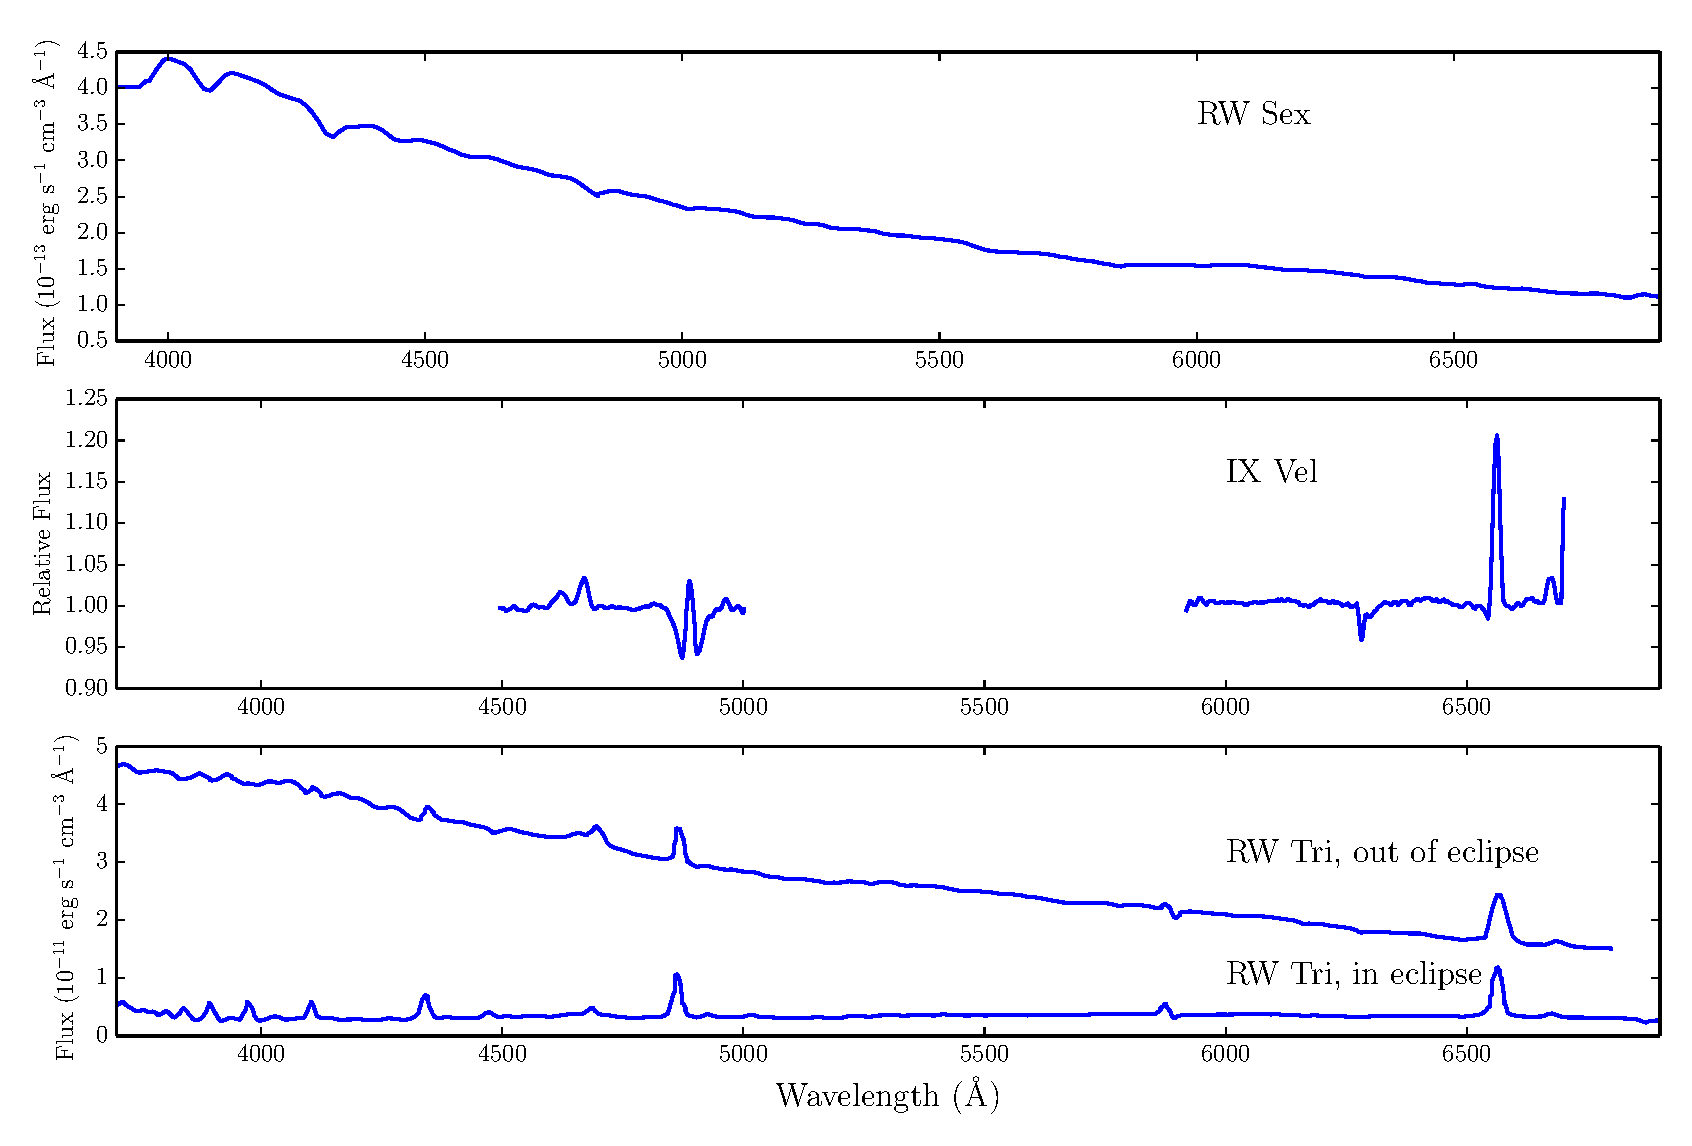
\includegraphics[width=0.8\textwidth]{figures/fig1.eps}
\caption{Optical spectra of three nova-like variables: 
RW Sex (top; Beuermann et al. 1992),
IX Vel (top middle; Beuermann \& Thomas 1990) 
and RW Tri in and out of eclipse (bottom two panels; Groot et al. 2004).
The data have been digitized from the respective publications and a few of the more
prominent emission and absorption lines are marked. 
These systems have inclinations of $30^\circ$, $60^\circ$ and $70^\circ$ 
respectively.
The trend of increasing Balmer line emission with inclination can be seen.
In RW Tri strong single-peaked emission in the Balmer lines is seen even
in eclipse, indicating that the lines may be formed in a spatially
extensive disk wind, and there is even a suggestion 
of a (potentially wind-formed) recombination continuum in the eclipsed
spectrum.}
\label{novalikes}
\end{figure}

%% CITATIONS FROM CAPTION
\nocite{groot2004}
\nocite{beuermann1990}
\nocite{beuermann1992}

Here, we carry out Monte Carlo radiative transfer simulations in
order to assess the likely impact of accretion disk winds on the
optical spectra of high-state CVs. More specifically, our goal is to
test whether disk winds of the type developed to account for the UV
resonance lines would also naturally produce significant amounts of  
optical line and/or continuum emission. In order to achieve this, we
have implemented the `macro-atom' approach developed by Lucy
(2002, 2003) into the Monte Carlo ionization and radiative transfer
code described by LK02 (a process initiated by SDL05). With this
upgrade, the code is able to deal correctly with processes involving
excited levels, such as the recombination emission produced by CV
winds. 

The remainder of this paper is organized as follows. In Section~2 we
briefly describe the code and and the newly implemented macro-atom
approach. In Section~3, we describe the kinematics and geometry of our
disk wind model. 
In Section~4, we present spectra simulated from the benchmark model
employed by LK02, and in Section~5, we carry out a limited sensitivity
study to explore how the predicted spectra change as a function of
some key parameters in our model. In Section~6, we summarize our
findings.


%%%%%%%%%%%%%%%%%%%%%%%%%%%%%%%%%%%%%%
%
%          THE CODE, RADIATIVE TRANSFER
%
%%%%%%%%%%%%%%%%%%%%%%%%%%%%%%%%%%%%%%%

\section{\sc{python}: A Monte Carlo Ionization and Radiative Transfer Code}

\py is a Monte Carlo (MC) ionization and radiative transfer code which
uses the Sobolev approximation to treat line transfer. It has already
been described extensively in LK02, SDL05 and H13, so here we provide
only a brief summary of its operation, focusing particularly on new
aspects of our implementation of macro-atoms into the code. 

\subsection{Basics} 

\py operates in two distinct stages. First, the ionization state,
level populations and temperature structure are calculated. This is
done iteratively, by 
propagating several populations of MC energy quanta (`photons')
through a model wind. The geometric and kinemetic properties of the
outflow are specified on a pre-defined spatial grid. In each of these
iterations (``ionization cycles''), the code records estimators that 
characterize the radiation field in each grid cell. At the end 
of each ionization cycles, a new electron temperature is calculated
that more closely balances heating and cooling in the 
plasma. The radiative estimators and updated electron
temperature are then used to revise the ionization state of the wind,
and a new ionization cycle is started. The process is repeated until
heating and cooling are balanced throughout the wind. 

This converged model is used as the basis for the second set of
iterations (``spectral cycles''). In these, the emergent spectrum over
the desired spectral range is synthesized by tracking populations of
energy packets through the wind and computing the emergent spectra at
a number of user-specified viewing angles.  

\py is designed to operate in a number of different
regimes, both in terms of the scale of the system, and in terms of the
characteristics of the underlying radiation field.
It was originally developed by LK02 in order to model the UV spectra
of CVs with a simple biconical disk wind model. Sim et al. (2005;
hereafter SDL05)\nocite{simmacro2005} used the code to model Brackett
and Pfund line profiles of H in young-stellar objects (YSOs). As part
of this effort, they implemented a `macro-atom' mode (see below) in
order to correctly treat hydrogen recombination lines with
\py. Finally, Higginbottom et al.\nocite{higginbottom2013} (2013;
hereafter H13) used \py to model broad absorption line (BAL) QSOs. For
this application, an improved treatment of ionization was implemented,
so that the code is now capable of dealing with arbritrary
photo-ionizing SEDs, including non-thermal and multi-component ones. 

\subsection{Ionization and Excitation: ``Simple Atoms''}
\label{simpleatoms}

Prior to SDL05, the relative ionization fractions for all atomic
species were estimated via the modified Saha equation (Mazzali \&
Lucy 1993)  
\begin{equation}
\frac{n_{j+1} n_e}{n_j} = W [\xi + W(1-\xi)]
\left(\frac{T_e}{T_R}\right)^{1/2}
\left(\frac{n_{j+1}n_e}{n_j}\right)^*_{T_R}, \label{ionization}
\end{equation}
Here, the `starred' term on the right represents abundances computed with
the Saha equation at temperature $T_R$, but using actual partition functions
from the dilute blackbody approximation. 
$W$ is an effective dilution factor, $\xi$ is the
fraction of recombinations going directly to the ground state, and
$T_R$ and $T_e$ are the radiation and electron temperature
respectively. This simple ionization scheme produces reasonable
results when the photoionizing SED can be approximated by a dilute
blackbody. This is the case for high-state CVs. (As noted above, an
improved, but more complex treatment of ionization that is appropriate
for more complex SEDs is described in H13.) 

Similarly, the relative excitation fractions within each ionization
stage of a given species were estimated via a modified Boltzmann
equation,
\begin{equation}
\frac{n_{jk}}{n_j} = \frac{W g_k}{z_j(T_R)} \exp(-E_k/kT_R),
\end{equation}
where $n_{jk}$ is the population of level $k$ in ionic stage $j$,
$E_k$ is the energy difference between level $k$ and the ground state,
and $z_j(T_R)$ is the partition function of ionic stage $j$. 

Finally, \py modelled all bound-bound processes as transitions
within a simple two-level atom \cite[see e.g.][]{mihalas}. This
approach works reasonable well for resonance  
lines, such as \civfull, in which the lower level is the ground state.  
However, it is a poor approximation for many other
transitions, particularly those where the upper level is 
is primarily populated from above. Thus an improved method for
estimating excited level populations and simulating line transfer is
needed in order to model recombination lines and continua.

\subsection{Ionization and Excitation: Macro-Atoms}

Lucy (2002, 2003\nocite{lucy2002, lucy2003}; hereafter L02, L03) 
has shown that it is possible to calculate the emissivity of a gas in
statistical equilibrium accurately by quantising matter into
`macro-atoms', and radiant and kinetic energy into indivisible energy
packets (r- and k- packets, respectively). His macro-atom scheme
allows for all possible transition paths from a given level and
provides a full non-local thermodynamic equilibrium (NLTE) solution
for the level populations based on MC estimators. The macro-atom
technique has already been used to model Wolf-Rayet star
winds \citep{sim2004}, AGN disk winds \citep{simlong2008, tatum2012},
supernovae \citep{kasen2006, kerzendorfsim} and YSOs (SDL05). A full 
description of the can be found in L02 and L03. 

Briefly, macro-atom NLTE level populations and ionization fractions
are calculated by solving the statistical equilbrium equations between
each pair of levels. For example, the bound-bound de-excitation rate,
${\cal R}_{ul}$, in an ion is given by  
\begin{equation}
{\cal R}_{ul} = \beta_{lu} A_{ul} n_u + \beta_{lu} B_{ul} n_u J_{lu} +
C_{ul} n_u n_e,\label{eq:nlte_rul},
\end{equation}
where $u$ and $l$ denote the upper and lower levels, $C$ represents the
collisional rate coefficients and $A$ and $B$ represent the Einstein
coefficients. The quantity $\beta_{lu}$ is the probability that a
given line photon will escape the Sobolev region. Finally, $J$ is the
MC estimator for the mean intensity in the line, as recorded during
the photon propagation. The corresponding excitation rate is then 
\begin{equation}
{\cal R}_{lu} = \beta_{lu} B_{lu} n_l J_{lu} + C_{lu} n_l n_e,
\end{equation}
where we implicitly include a correction for stimulated emission in
our definition of the estimate for $J_{ul}$. 

In our implementation of the macro-atom approach, we also explicitly
take into account the photoionization and collisional ionization rates
between a lower level, $l$, and the continuum (or, in the case of ions
with more than one bound electron, the ground state of the upper ion),
$\kappa$,
\begin{equation}
{\cal R}_{l \kappa}= n_l \int_{\nu_0}^{\infty} \frac{ 4 \pi J_{\nu}
  \sigma_{\nu}}{h \nu} d\nu + C_{l \kappa} n_l n_e.
\end{equation}

Here, $\sigma_{\nu}$ is the photoionization cross section, and $J_{\nu}$
is the mean intensity. The corresponding recombination rate is given
by 
\begin{equation}
{\cal R}_{\kappa l} = \alpha_{\kappa l} n_{\kappa} n_e + C_{\kappa l}
n_\kappa n_e, \\
\end{equation}
where $\alpha_{\kappa l}$ is the radiative recombination coefficient
to level $l$. This treatment means that radiative and collisional
rates to and from all levels are considered when calculating both the
ionization state and the level populations, although we neglect 
ionization directly to excited levels of the upper ion. The
\cite{vanregemorter} approximation is used for collisional
transitions, and thus we assume that collisions between radiatively
forbidden transitions are not important in determining level
populations. This is a reasonable approximation in the regimes
considered here.

\subsection{Ionization and Excitation: A Hybrid Approach}

SDL05 implemented a macro-atom treatment of Hydrogen in \py and used
this to predict the observable properties of a pure Hydrogen wind
model for YSOs. Our goal here is to simultaneously model the optical
and ultraviolet spectra of high-state CVs. Since the optical spectra
are dominated by H and He recombination lines, both of these species
need to be treated as macro-atoms. The UV spectra, on the other hand,
are dominated by resonance lines associated with metals. This means we
need to include these species in our models, but they can be treated 
with our (much faster) simple-atom approach. We have therefore
implemented a hybrid ionization and excitation scheme into \py. Any
atomic species can now be treated either in our simple-atom
approximation or with the full macro-atom machinery. For our CV
models, we treat H and He as macro-atoms and all metals as
simple-atoms.  

\subsection{Atomic Data}

We generally use the same atomic data as H13, which is an updated
version of that described in LK02. In addition, we follow SDL05 in
treating Hydrogen as a 20-level atom, where each level is defined by
the principal quantum number, $n$. For the macro-atom treatment of
Helium,  we have added additional level and line information required 
from \textsc{Topbase} \citep{topbase2005}.  He~\textsc{II} is treated
in much the same way as H, but with 10 levels. He~\textsc{I} has
larger energy differentials between different l-subshells and triplet
and singlet states. Thus, we still include levels up to $n=10$ but
explicitly treat the $l$ and $s$ sub-orbitals as distinct levels
instead of assuming they are perfectly `l-mixed'. This allows us
to model the singlet and  triplet He~\textsc{i} lines that are ubiquitous
in the optical spectra of CVs \citep[e.g.][]{dhillon1996}.


\subsection{Code Validation and Testing}

\py has been tested against a number of radiative transfer and
photoionization codes. LK02 and H13 conducted comparisons of 
ionization balance  with \cld \citep{cloudy2013}, demonstrating
excellent agreement. We have also carried out comparisons
of ionization and spectral synthesis with the supernova code
\textsc{Tardis.} \tar is described by 
\cite{kerzendorfsim}, and the spectral comparisons can be found
therein. For the effort reported here, we have additionally carried
out tests of the macro-atom scheme in \py. Figure~\ref{tests} shows
two of these tests. In the top panel, we compare the Balmer series 
emissivities as predicted by \py in the l-mixed Case~B limit against the
analytical calculations by \cite{seaton1959}. In the bottom panel, we
compare \py and \tar predictions of  He \textsc{i} level populations
for a particular test case. Agreement is excellent for both H and He.

\begin{figure}
\centering
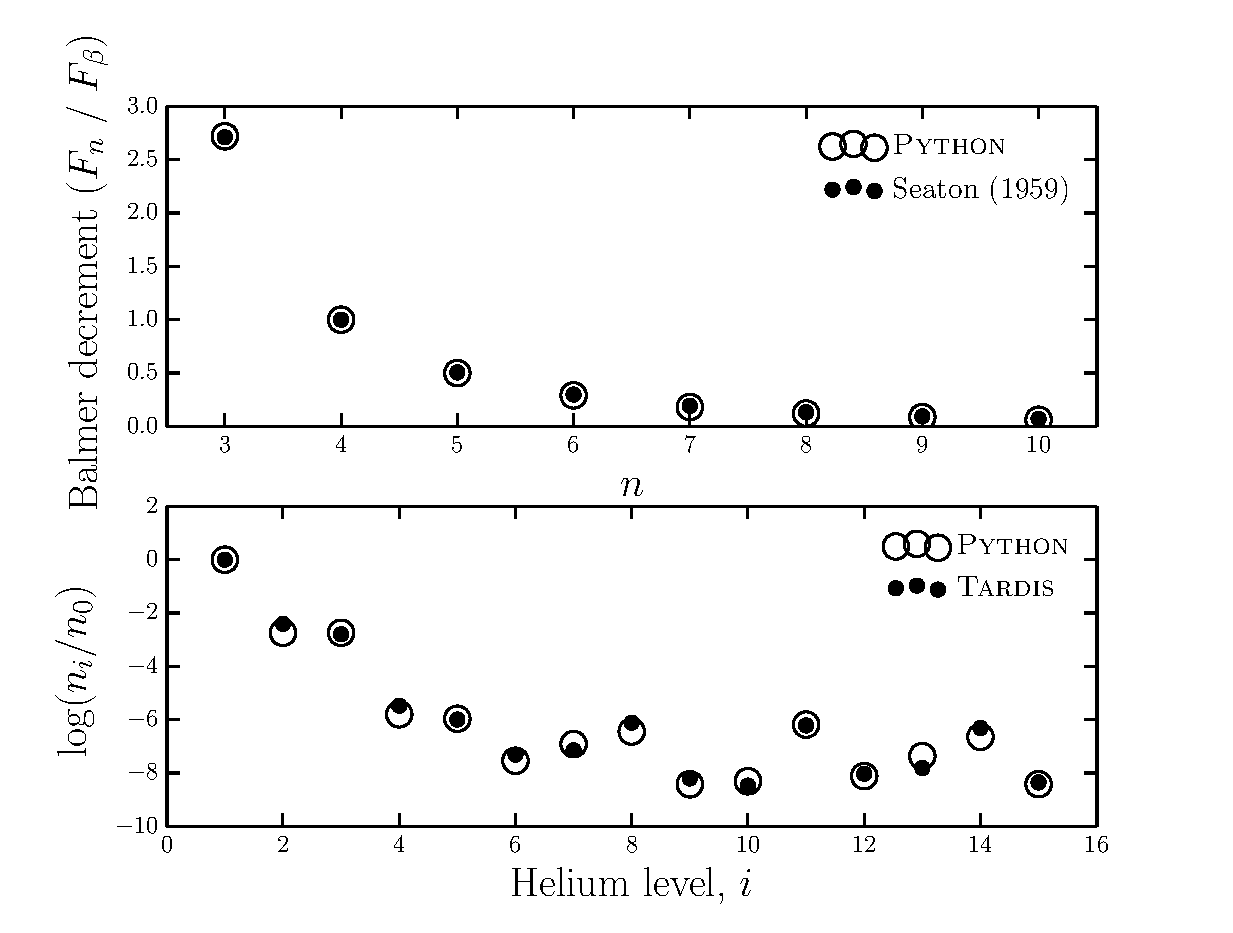
\includegraphics[width=0.5\textwidth]{figures/fig_caseb_tardis.eps}
\caption{
{\sl Top Panel:} ``Case B'' Balmer decrements computed 
with \textsc{Python} compared to analytic calculations
by Seaton (1959). Both calculations are calculated at $T_e=10,000$K.
(see Osterbrock 1989 for a discussion of this commonly used approximation).
{\sl Bottom Panel:}  a comparison of Helium I level populations (the most complex ion we currently 
treat as a macro-atom) between \py~and \tar~models. 
The calculation is conducted with physical parameters of $n_e=5.96\times10^4$~cm$^{-3}$,
$T_e=30,600$K, $T_R=43,482$K and $W=9.65\times10^{-5}$. 
Considering the two codes use different atomic data and \textsc{Tardis,} unlike \textsc{Python,} currently has a complete treatment of collisions between 
radiatively forbidden transitions, the factor of 
$<2$ agreement is encouraging. 
}
\label{tests}
\end{figure}


\nocite{osterbrock}
\nocite{seaton1959}

%%%%%%%%%%%%%%%%%%%%%%%%%%%%%%%%%%%%%%
%
%          THE MODEL
%
%%%%%%%%%%%%%%%%%%%%%%%%%%%%%%%%%%%%%%%

\section{Describing the System and its Outflow}

\py includes several different kinematic models of accretion disk
winds, as well as different options for describing the physical and
radiative properties of the wind-driving system under
consideration. Most of these features have already been discussed in
LK02 and H13, so below we only briefly recount the key aspects of the
particular system and wind model used in the present study.

\subsection{Wind Geometry and Kinematics}
\label{kinematics}

We adopt the kinematic disk wind model developed by Schlosman \&
Vitello (1993; hereafter SV93). A schematic of this model is shown in
figure~\ref{cartoon}. In this parametrization, a smooth, biconical
disk wind emanates from the accretion disk between radii $r_{min}$ and 
$r_{max}$. The covering fraction of the outflow is also controlled by the
inner and outer opening angles of the wind, $\theta_{min}$ and
$\theta_{max}$, and the launch angle of the other streamlines is given
by 
\begin{equation}
\theta(r_0) = \theta_{min} + (\theta_{max} - \theta_{min}) \left(\frac{r_0 - r_{min}}{r_{max} - r_{min}} \right)^{\gamma},
\label{theta}
\end{equation}
where $r_0$ is the launch radius of the streamline.

The poloidal (non-rotational) velocity field of the wind, $v_l$, is given by
\begin{equation}
v_l=v_0+\left[v_{\infty}(r_0)-v_0\right]\frac{\left(l/R_v\right)^{\alpha}}{\left(l/R_v\right)^{\alpha}+1},
\label{v_law}
\end{equation}
where $l$ is the poloidal distance along a particular wind
streamline. The terminal velocity along a streamline, $v_{\infty}$, is
set to a fixed multiple of the escape velocity at the launch
point. The launch velocity from the disk surface, $v_0$, is assumed to
be constant (set to $6$~km~s$^{-1}$). Once the wind is launched, it
accelerates, reaching half of its terminal velocity at $l = R_v$. The
velocity law exponent $\alpha$ controls how quickly the wind
accelerates. Larger values of $\alpha$ cause the main region of 
acceleration to occur close to $R_v$, whereas smaller values
correspond to fast acceleration close to the disk (see
figure~\ref{acc_law}). 


\begin{figure}
\centering
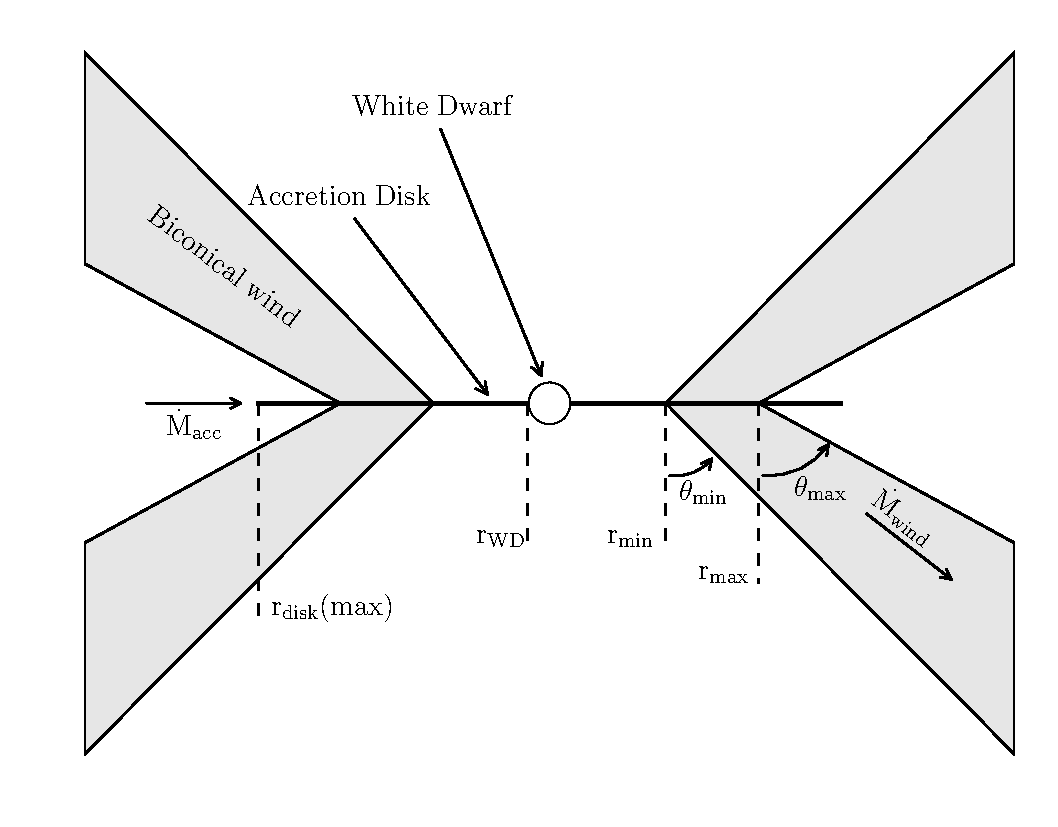
\includegraphics[width=0.5\textwidth]{figures/fig2_cartoon.eps}
\caption{Cartoon illustrating the geometry and kinematics of the benchmark CV wind model.}
\label{cartoon}
\end{figure}

\begin{figure}
\centering
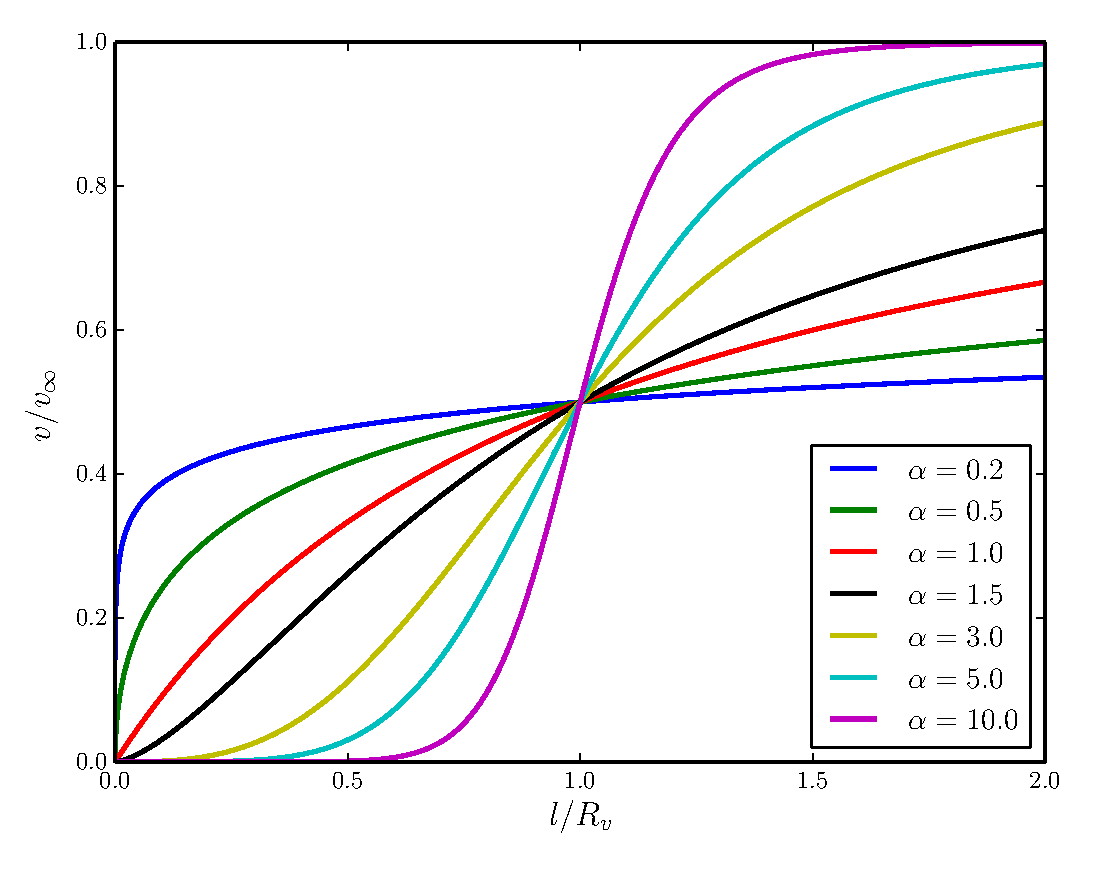
\includegraphics[width=0.45\textwidth]{figures/acc_law.eps}
\caption{
The adopted poloidal velocity law for various values of the
acceleration exponent, $\alpha$.} 
\label{acc_law}
\end{figure}

The density at position $(r,z)$ in the wind, $\rho(r,z)$, is
calculated from the mass continuity equation, yielding
\begin{equation}
\rho(r,z) = \frac{r}{r_0} \frac{dr}{dr_0} \frac{\phi(r_0)}{v_z(r,z)}.
\label{density}
\end{equation}
Here, $\phi(r_O)$ is the mass-loss rate per unit area at $r_0$, 
and $v_z$ is the vertical velocity component. We take $\phi(r_0)$ to be
uniform across the wind-launching area of the disk and normalize it by
matching its integral to the user-specified total mass-loss rate,
$\dot{M}_{wind}$. 
{\bf CK: I'm still not sure I understand the formula
  SV93 use to define $\phi$, and hence that this description is
  actually strictly correct.... Not sure what to do about that
  though...}

\subsection{Sources and Sinks of Radiation}
\label{radsources}

The net photon sources in our CV model are the accretion disk, the
WD and, in principle, a boundary layer with user-defined temperature
and luminosity. All of these radiating bodies are taken to be
optically thick, and photons striking them are assumed to be destroyed
instantaneously. The secondary star is not included as a radiation
source, but is included as an occulting body. This allows us to model
eclipses. Finally, emission from the wind itself is also accounted for, but
note that we assume the outflow to be in radiative equilibrium. Thus all
of the heating of the wind, as well as its emission, is ultimately
powered by the radiation field of the net photon sources in the
simulation. In the following sections, we will describe our treatment
of these system components in slightly more detail.

\subsubsection{Accretion Disk}

\py has has some flexibility when treating the accretion 
disk as a source of photons. The disk is broken down into annuli 
such that each annulus contributes an equal amount to the bolometric
luminosity. We take the disk to be geometrically thin, but optically
thick and thus adopt the temperature profile of a standard
\cite{shakurasunyaev1973} $\alpha$-disk. An annulus can then
be treated either as a blackbody with the corresponding effective
temperature or as a stellar atmosphere model with the appropriate
surface gravity and effective temperature. Here, we use blackbodies 
during the ionization cycles and to compute our MC
estimators. However, during the spectral synthesis stage of the 
simulation we use stellar atmosphere models. This produces more
realistic model spectra and allows us to test if recombination
emission from the wind base can fill in the Balmer jump, which is
always in absorption in these models. Our synthetic stellar atmosphere
spectra are calculated with
\textsc{Synspec}\footnote{http://nova.astro.umd.edu/Synspec43/synspec.html}
from either Kurucz \citep{kurucz1991} atmospheres (for $T_{eff} \leq
50,000$~K) or from \textsc{TLUSTY} models \citep{tlusty} (for $T_{eff} > 50,000$~K). 

\subsubsection{White Dwarf}

The WD at the center of the disk is always present as a spherical occulting
body with radius $R_{WD}$ in \py CV models, but it can also be included
as a source of radiation. In the models presented here, we treat the
WD as a blackbody radiator with temperature $T_{WD}$ and luminosity
$L_{WD} = 4\pi R_{WD}^2 \sigma T_{WD}^4$. 

\subsubsection{Boundary Layer}

It is possible to include radiation from a boundary layer (BL) between
the disk and the WD. In \py, the BL is described as
a blackbody with a user-specified effective temperature and
luminosity. In the models presented here, we have followed LK02 in setting
the BL luminosity to zero. However, we have confirmed that the addition of a
BL with $L_{BL} = 0.5 L_{acc}$ and temperatures in the range $80{\rm
kK} \leq T_{BL} \leq 200{\rm kK}$ would not change any of our main
conclusions. 
{\bf CK: Is this true? Do we want to say anything else, e.g. that we'll
talk about this in a future paper? JM: This is true. Anything up to 200kK
still has optical lines. The He II behaviour is not monotnic. CIV drops
gradually and gets a little overionized- but this is a separate topic really.
The issue of clumping and BL and their affect on ionization could be a 
future paper.}  

\subsubsection{Secondary Star}

The donor star is included in the system as a pure radiation sink, 
i.e. it does not emit photons, but absorbs any photons that strike its
surface. The secondary is assumed to be Roche-lobe filling, so its
shape and size are defined by setting the mass ratio of the system, $q
= M_2/M_{WD}$. The inclusion of the donor star as an occulting body
allows us to model eclipses of the disk and the wind. For this
purpose, we define orbital phase such that $\Phi_{orb} = 0$ as the
inferior conjunction of the secondary (i.e. mid-eclipse for $i \simeq
90^o$).

\begin{figure}
\centering
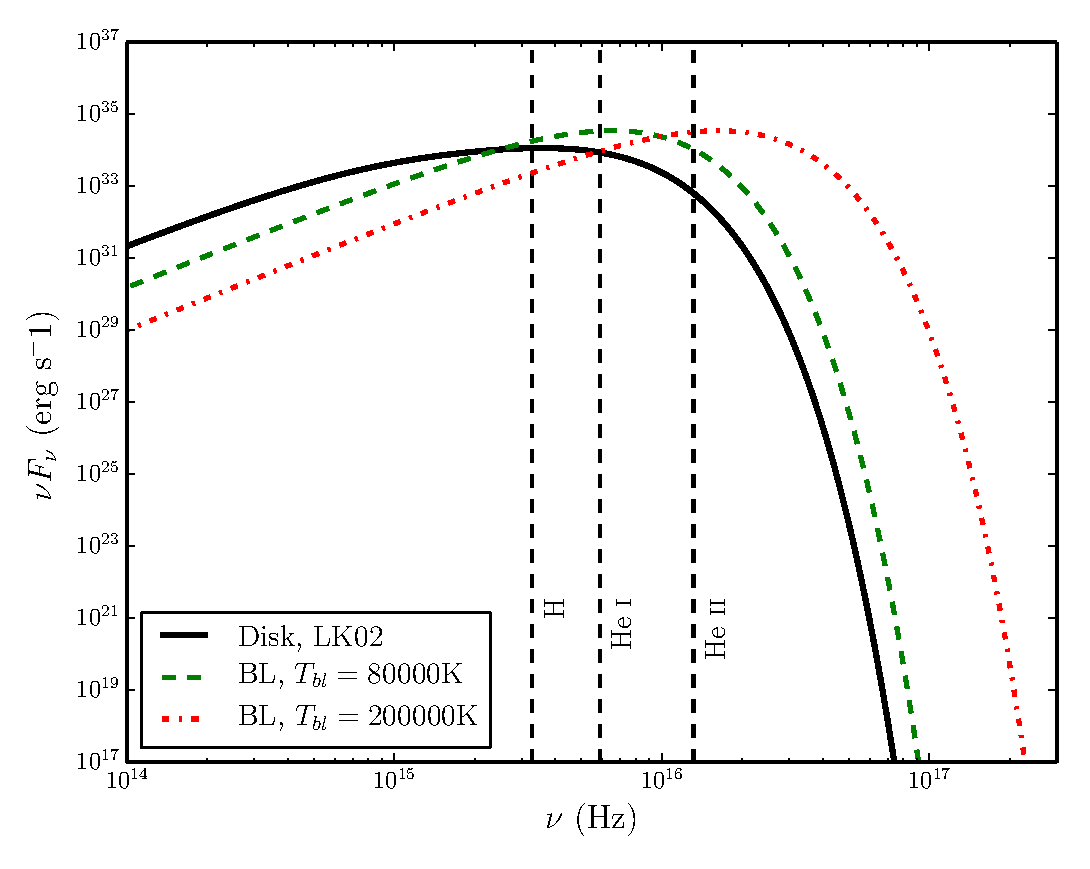
\includegraphics[width=0.45\textwidth]{figures/sed_figure.eps}
\caption{
The spectral energy distribution (SED) of the 
White Dwarf (dashed line) and blackbody accretion
disk used in the ionization calculation (black solid line).
The positions of the Hydrogen and Helium ionization edges 
are marked with vertical lines.
{\bf JM: do we want to show the stellar atmosphere spectrum here?
we know it looks a bit crap around the He II edge, so perhaps not...
 }
 }
\label{sed}
\end{figure}


%%%%%%%%%%%%%%%%%%%%%%%%%%%%%%%%%%%%%%
%
%          RESULTS
%
%%%%%%%%%%%%%%%%%%%%%%%%%%%%%%%%%%%%%%%




\begin{table}
\centering
\begin{tabular}{p{2cm}p{2cm}p{2cm}}
Model Parameters \\
\hline Parameter 	&	 Model A  & Model B \\ 
\hline \hline 
$M_{WD}$ 	 &	 $0.8 M_{\odot}$  &     \\ 
$R_{WD}$ 	 &	 $7\times10^{8}$cm  & \\ 
$T_{WD}$ 	 &	 $40,000$K        &  \\
$M_{2}$ 	 &	 $0.6 M_{\odot}$  &   \\ 
$\dot{M}_{acc}$ 	 &	 $10^{-8}~M_{\odot}yr^{-1}$  &\\ 
$\dot{M}_{wind}$  &	$10^{-9}~M_{\odot}yr^{-1}$å  & \\ 
$r_{min}$ 	&	 $4 R_{WD}$ &  \\ 
$r_{max}$ 	&	 $12 R_{WD}$  &  \\ 
$\theta_{min}$ 	&	 $20.0^{\circ}$  &  \\ 
$\theta_{max}$ 	&	 $65.0^{\circ}$  &  \\ 
$\gamma$ 	&	 $1$  &  \\ 
$v_{\infty}$ 	&	 $3v_{esc}$  &  \\ 
%%$R_v$ 	        &	 $7\times10^{10}$cm \\ 
$R_v$ 	        &	 $100 R_{WD}$  &  $142.9 R_{WD}$  \\ 
$\alpha$ 	&	 $1.5$   &   $4$\\
\end{tabular}
\centering
\caption{
Parameters used for the geometry and kinematics of the benchmark 
CV model (Model A), which is optimized for the UV band, and a model
which is optimized for the optical band and described in section 6 (Model B).
For Model B, only parameters which are altered are given - otherwise the
Model A parameter is used.
{\bf JM: this needs some stuff adding, as is mentioned in certain places}}
\label{wind_param}
\label{modelb_table}
\end{table}

\section{A Benchmark Disk Wind Model}
\label{modela}

Our main goal is to test whether the type of disk wind model that has
been successful in explaining the UV spectra of CVs could also have 
significant impact on the optical continuum and emission line spectra
of these systems. In order to set a benchmark, we therefore begin by
investigating one of the fiducial CV wind models that was used by SV93
and LK02 to simulate the UV spectrum of a typical high-state
system. The specific parameters for this model (Model A) are listed in
Table~1. A key point is that the wind mass-loss rate in this model is
set to 10$\%$ of the accretion rate through the disk.

\subsection{Physical Structure and Ionization State}
\label{modela_ionization}

\begin{figure} %fullpage
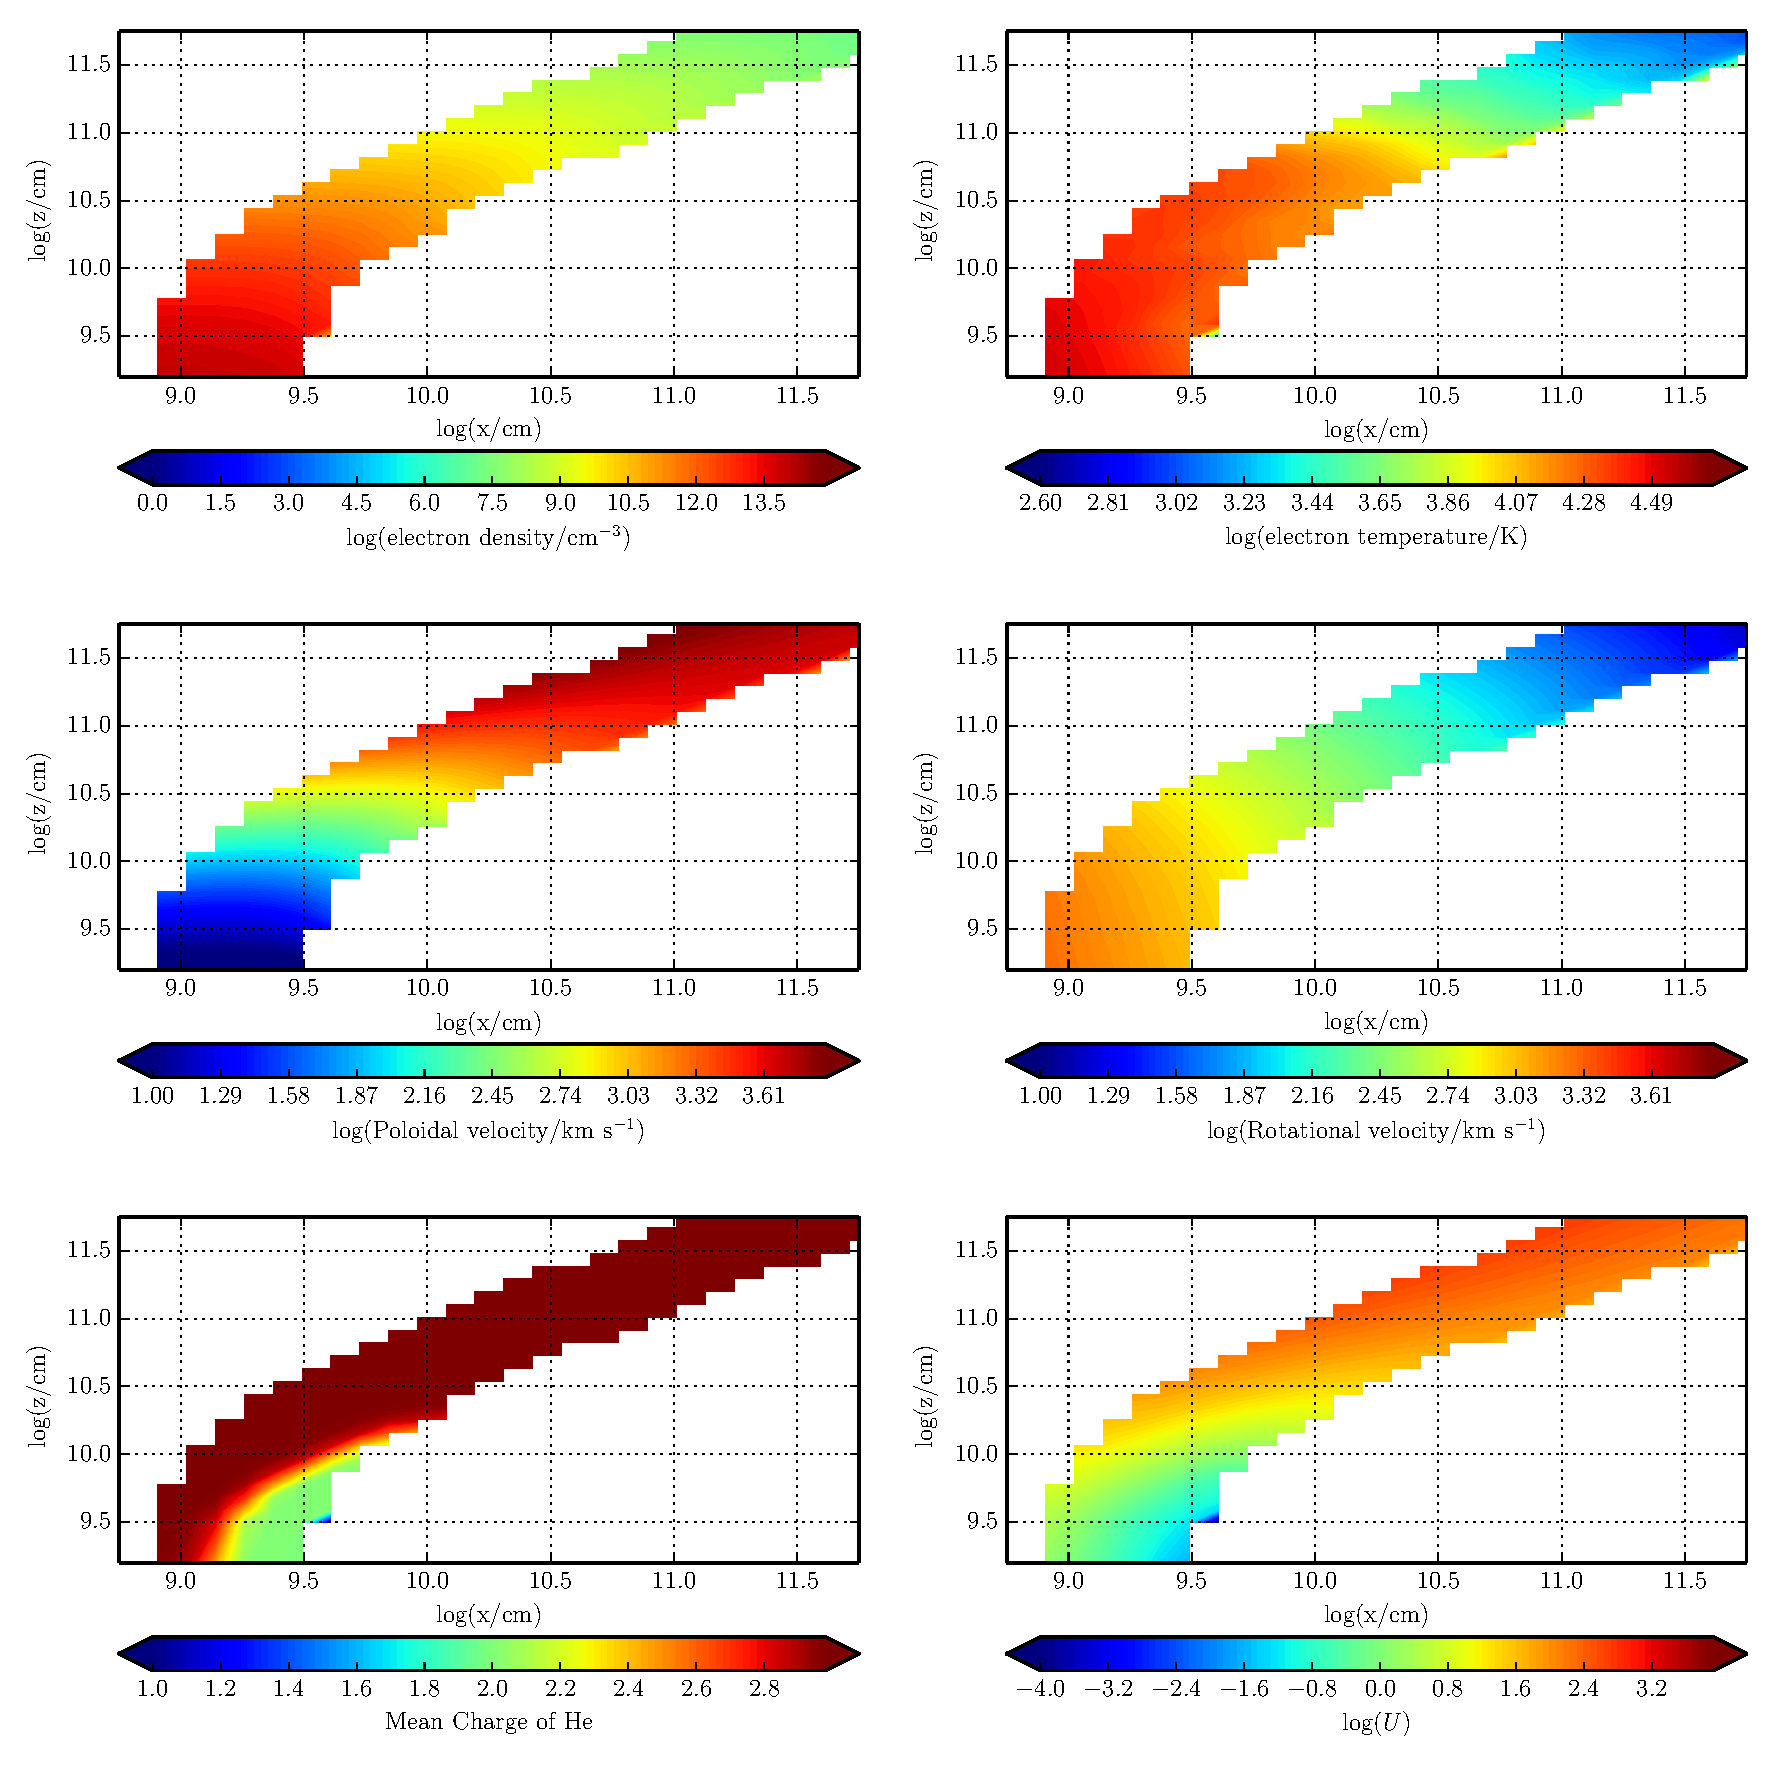
\includegraphics[width=\textwidth]{figures/fig5.eps}
\caption{
The physical properties of the wind- note the logarithmic scale. 
Near the disk plane the wind is dense, with low poloidal velocities.
As the wind accelerates it becomes less dense
and more highly ionized. The dominant Helium ion
is almost always He III, apart from in a small
portion of the wind at the base, which is partially shielded
from the inner disk.
}
\label{wind}
\end{figure} %fullpage

Figure~\ref{wind} shows the physical and ionization structure 
of the benchmark disk wind model. There is an obvious drop-off in density
and temperature with distance away from the disk, so any line
formation process that scales as $n_e^2$ - i.e. recombination and
collisionally excited emission - should be expected to operate
primarily in the dense base of the outflow. Moreover, a comparison of
the rotational and poloidal velocity fields shows that rotation
dominates in the near-disk regime, while outflow dominates further out
in the wind. 

The ionization equation used in the ``simple atom'' approach used in
LK02 (see section~\ref{simpleatoms}) should be a reasonable approximation to
the photoionization equilibrium in the benchmark wind model. Even
though the macro-atom treatment of H and He does affect the 
computation of the overall ionization equilibrium, we would expect the
resulting ionization state of the wind to be quite similar to that
found in LK02. The bottom panels in figure~\ref{wind} confirm that this
is the case. In particular, Helium is fully ionized
throughout most of the outflow, except for a small region near the
base of the wind, which is shielded from the photons produced by the
hot inner disk. In line with the results shown in LK02, we also find
that C\textsc{iv} is the dominant Carbon ion throughout the wind,
resulting in a substantial absorbing column across a large range of
velocities. As we shall see, this produces the broad, deep and
blue-shifted C\textsc{iv}~$\lambda 1550{\rm \AA}$ absorption line that
is usually the most prominent wind-formed feature in the UV spectra of
low-inclination nova-like CVs.

\subsection{Synthetic Spectra}
\label{modela_spectrum}

We begin by verifying that the benchmark model still produces UV
spectra that resemble those observed in CVs. We do expect this to be
the case, since the ionization state of the wind has not changed
significantly from that computed in LK02 (see section~\ref{modela_ionization}). 
The left column of panels in figure~\ref{spec} shows that this expectation
is met: all of the strong metal resonance
lines - notably N\textsc{v}~$\lambda 1240{\rm \AA}$,
Si\textsc{iv}~$\lambda 1400{\rm \AA}$ and C\textsc{iv}~$\lambda
1550{\rm \AA}$ - are present and exhibit clear P-Cygni profiles
at intermediate inclinations. In addition, however, we now also find
that the wind produces significant Lyman-$\alpha$ and
He~\textsc{ii}~$\lambda1640{\rm \AA}$ emission lines. 

\begin{figure} %fullpage
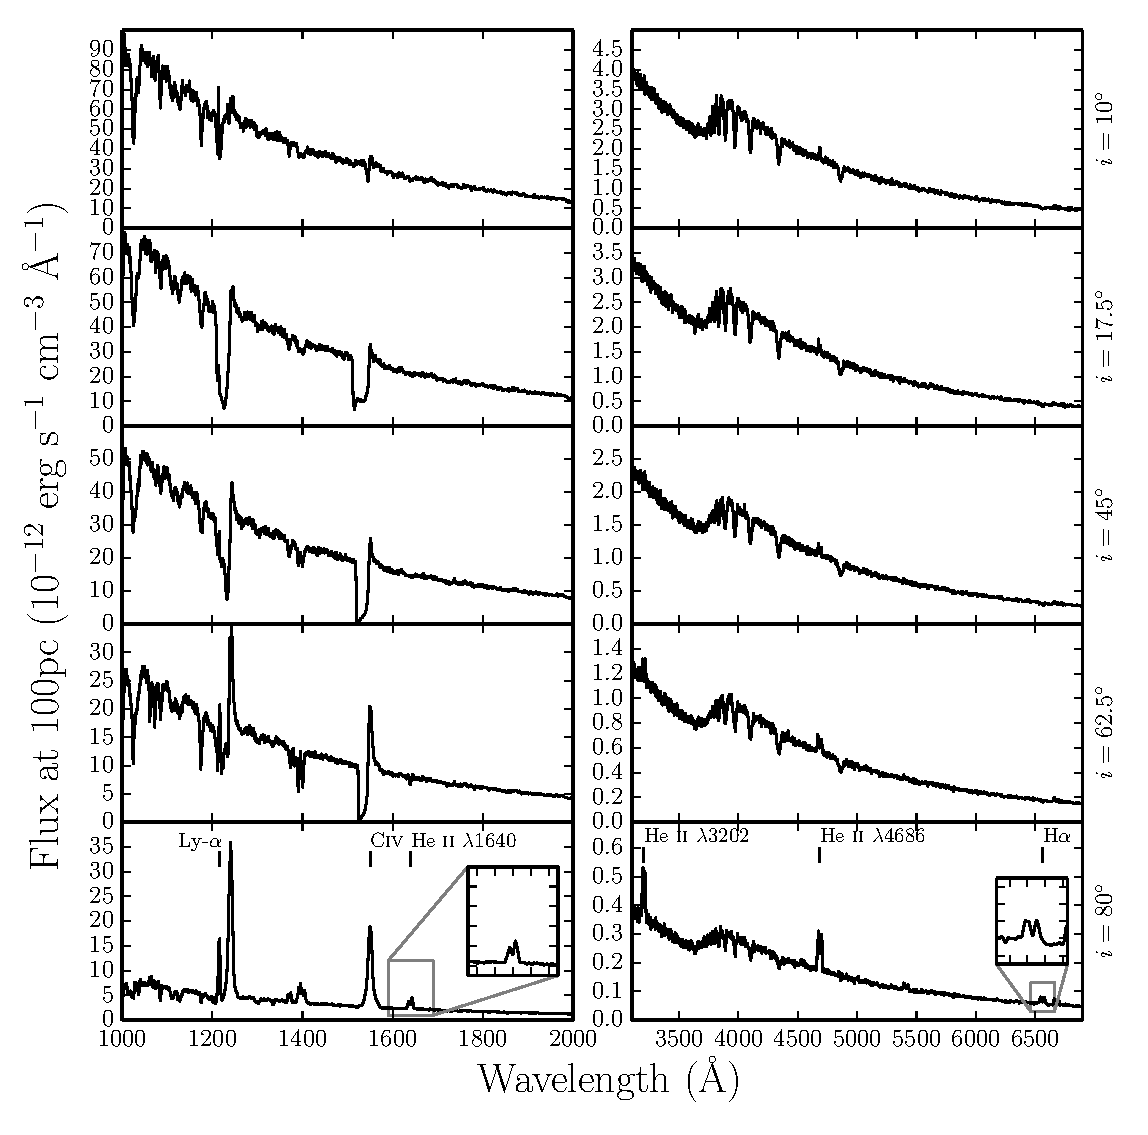
\includegraphics[width=\textwidth]{figures/fig5_uv_opt.eps}
\caption{
UV (left) and optical (right) synthetic spectra for model A, our benchmark model,
computed at sightlines of 10, 27.5, 45, 62.5 and 80 degrees.	
The inset plots show zoomed-in line profiles for 
\heiiuv\ and \ha. Double-peaked line emission can be seen in 
\heiiuv, \heiiopt, \ha\ and some He I lines, but the 
line emission is not always sufficient to overcome the absorption
cores from the stellar atmosphere models. The model
also produces a prominent \heiioptnew\ line at high inclinations,
}
\label{spec}
\end{figure} %fullpage\

Figure~\ref{spec} shows the corresponding optical spectra produced for
the benchmark model, and these do exhibit some emission lines
associated with H and He. Since the emissivity of these recombination 
features scales as $n_e^2$, they are formed almost entirely in the 
dense base of the wind, just above the accretion disk. Here, the
velocity field of the wind is still dominated by rotation, rather than
outflow, which accounts for the double-peaked shape of the lines. In
principle, lines formed in this region can still be single peaked,
since the existence of a poloidal velocity {\em gradient} changes the
local escape probabilities (MC96). However, as
demonstrated explicitly in section~\ref{modelb}, the line opacity in our
benchmark model is not high enough for this radiative transfer effect
to dominate the line shapes.

We also see a general trend from absorption lines to emission lines 
with increasing inclination, as one might expect from our wind
geometry. This trend is consistent with observations, as can be seen
in Figure~1.

The Balmer jump is in absorption at all inclinations for our benchmark
model. This is due to the stellar atmospheres we have used to
model the disk spectrum; it is not a result of photoabsorption in the
wind. In fact, the wind spectrum exhibits the Balmer jump in {\em
emission}, but this is not strong enough to overcome the intrinsic
absorption edge in the disk spectrum. This is illustrated in
Figure~\ref{cont}, which shows the angle-integrated spectrum of the system,
i.e. the spectrum formed by all escaping photons, separated into the
disk and wind contributions. Even though the wind-formed Balmer
recombination continuum does not completely fill in the Balmer
absorption edge in this model, it does already contribute
significantly to the total spectrum. This suggests that modest changes 
to the outflow kinematics might boost the wind continuum and produce
emergent spectra with weak or absent Balmer absorption edges. 

\begin{figure} 
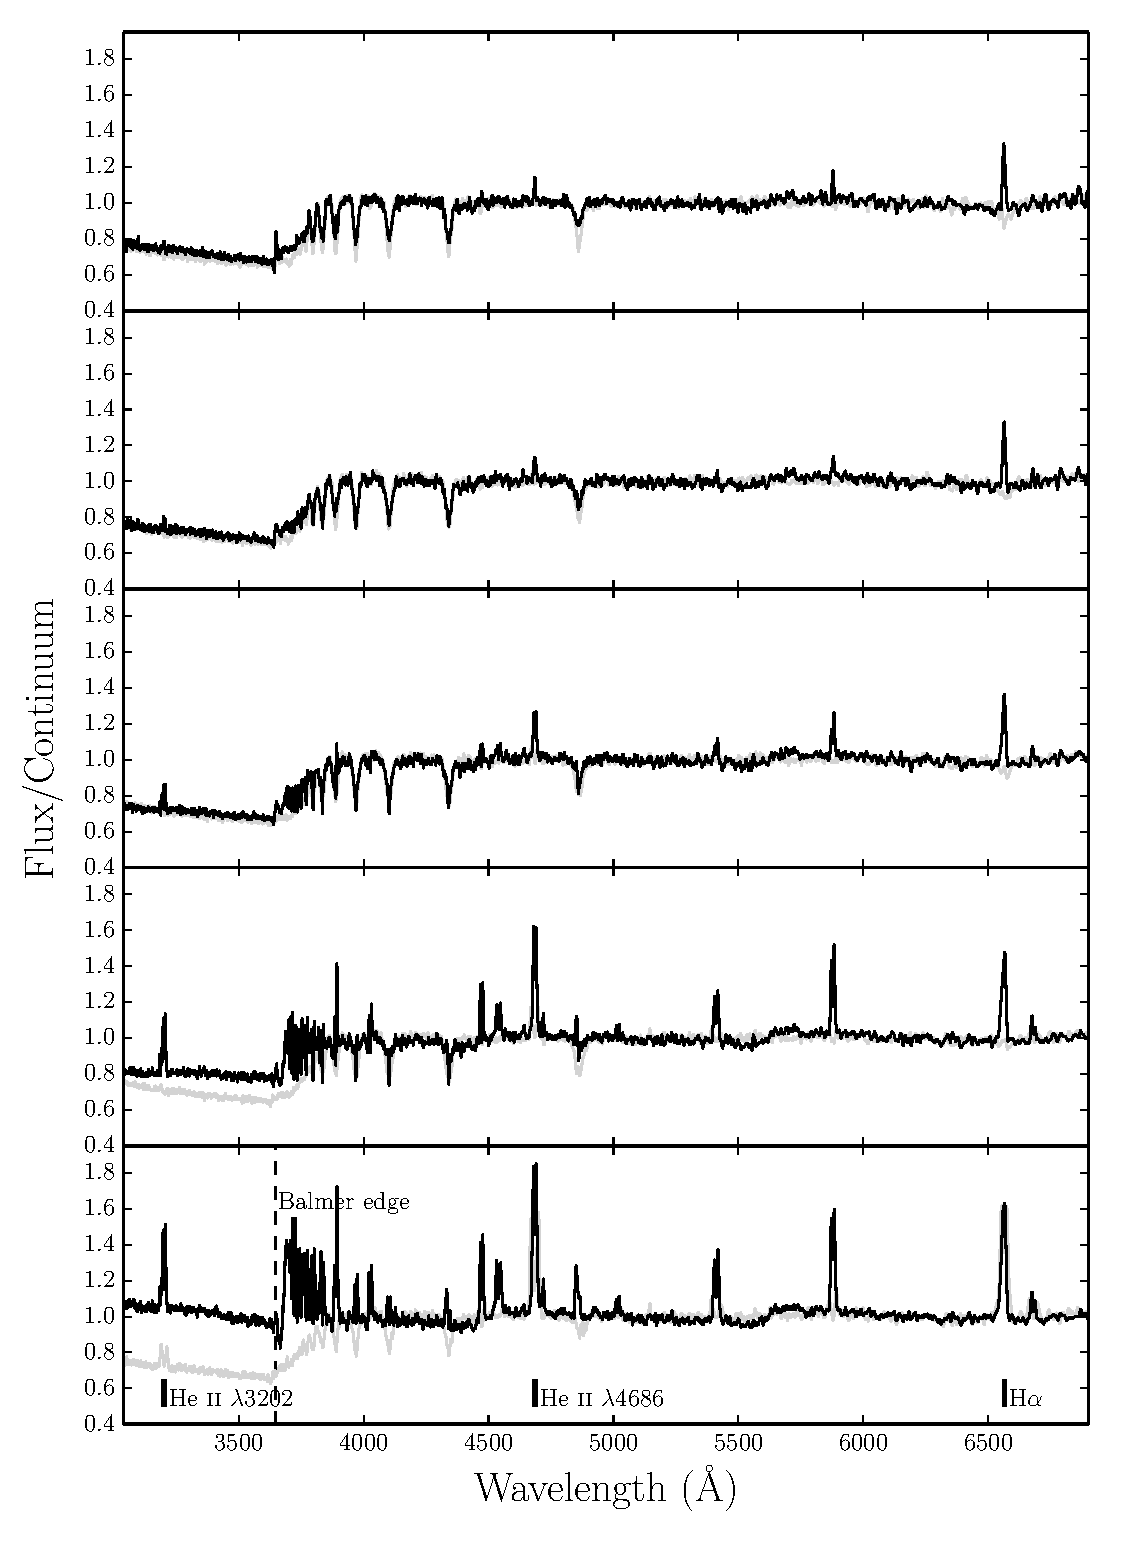
\includegraphics[width=0.45\textwidth]{figures/fig6_opt_cont.eps}
\caption{Synthetic optical spectra computed for 
sightlines of 22.5, 25, 62.5 and 80 degrees. In these plots
the flux is divided by a polynomial fit to the 
underlying continuum redward of the Balmer edge, so that 
line-to-continuum ratios and the true depth of the
Balmer jump can be shown.}
\label{spec_continuum}
\end{figure} 

\begin{figure} 
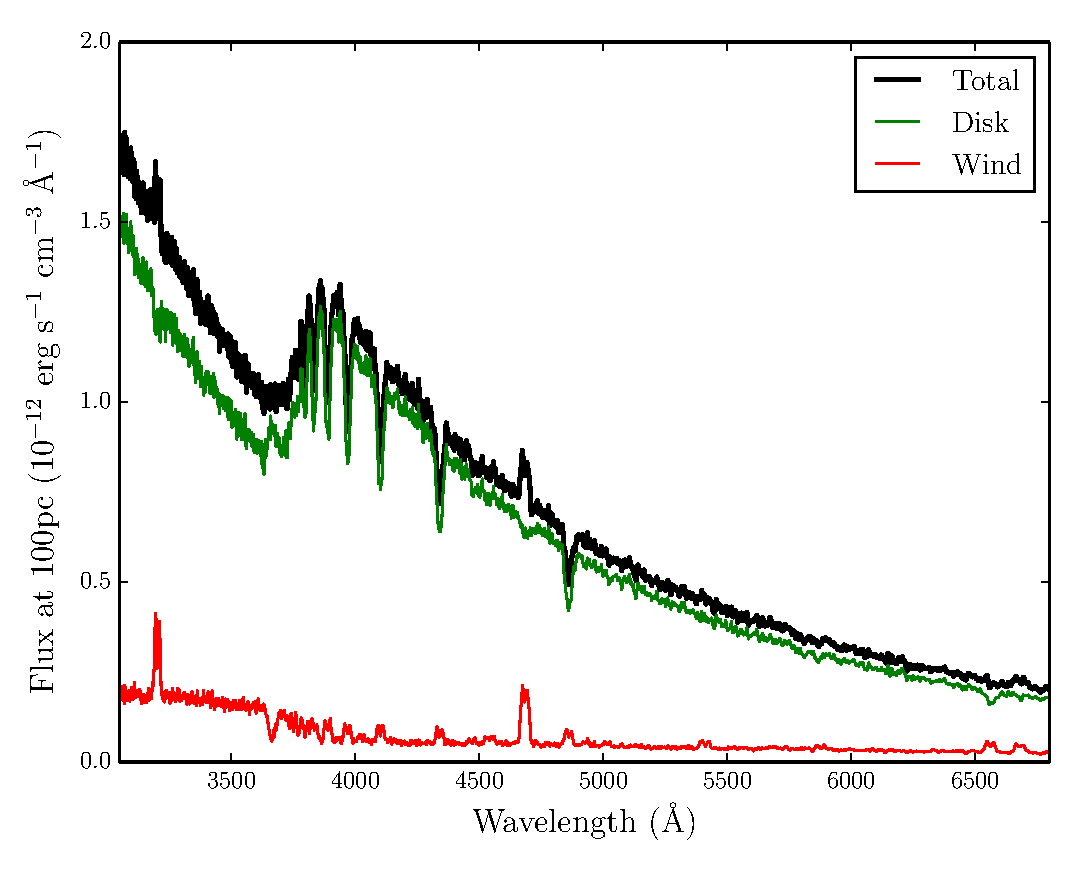
\includegraphics[width=0.5\textwidth]{figures/fig7_escaping.eps}
\caption{Total packet-binned spectra across all viewing angles. 
The thick black line shows the total 
integrated escaping spectrum, while green and red lines show the contributions from photons that originate in the disk and wind respectively. 
Recombination continuum emission blueward of the Balmer 
edge is already prominent relative to other wind continuum processes, but is not sufficient
to fill in the Balmer jump in this specific model}
\label{cont}
\end{figure} 





%%%%%%%%%%%%%%%%%%%%%%%%%%%%%%%%%%%%%%
%
%          DISCUSSION
%
%%%%%%%%%%%%%%%%%%%%%%%%%%%%%%%%%%%%%%%

\section{The Dependence of Wind Features on Outflow Parameters}
\label{modelb}

The results of section~\ref{modela} show that wind models that reproduce
the UV spectral features of CVs are likely to leave a clear imprint on
the optical spectrum. It is therefore important to understand the
sensitivity of optical (and UV) wind-formed features to the basic
properties of the outflow. In particular, there are two key questions
we would like to address: (i) under what conditions can disk winds
produce {\em single-peaked} Balmer emission lines (MC96); (ii) can the wind-formed recombination continuum completely
fill in the disk's Balmer absorption edge for reasonable outflow
parameters? 

The amount of recombination and collisionally excited emission
produced by a given ion, $i$, in a plasma of volume $V$ depends
primarily on the emission measure, $EM$, defined as 
\begin{equation}
EM=\int^V_0 n_e n_i \,dV,
\end{equation}
where $n_i$ is the number density of the ion in question.    
The emission reaching an observer at a given frequency also depends on
the Sobolev optical depth it experiences, which depends on both the
density and the velocity gradient projected along the line of
sight. This can also significantly affect line profile shapes. 

The simplest way to simultaneously affect the density in the wind as
well as the velocity gradients is by modifying the poloidal velocity
law. We have therefore conducted a exploratory sensitivity study in
which we focus on just two kinematic variables (section~\ref{kinematics}):

\begin{itemize}
 	\item the acceleration length, $R_v$, which controls the
        distance over which the wind accelerates to $\frac{1}{2}v_{\infty}$;
 	\item the acceleration exponent, $\alpha$, which controls the rate 
 	at which the poloidal velocity changes near $R_v$.
\end{itemize} 
The general behaviour we might expect is that outflows with denser
regions near the wind base -- i.e. winds with larger $R_{v}$ and/or
larger $\alpha$ -- will produce stronger optical emission signatures. 
However, this behaviour may be moderated by the effect of the increasing
optical depth through this region.

\subsection{Optical Wind Signatures}
\label{modelb_opt}

Figure~\ref{halpha} shows how the H$\alpha$ and 
He~{\sc ii}~$\lambda 
4686$ lines change with the kinematics of the wind for an inclination
of $80^\circ$. The width and strength of He~{\sc ii} clearly depend on
both $R_v$ and $\alpha$, but the overall line profile shape is always
double-peaked. This contrasts with the behaviour of H$\alpha$, which
becomes single-peaked in our densest models. The transition from
double-peaked to single-peaked occurs when the line becomes optically
thick. This reproduces the behaviour predicted by \cite{MC96}, who
showed that the poloidal velocity gradient in the wind can modify the
shape of optically thick emission lines even in the near-disk regime,
where the poloidal velocity itself is much smaller than the rotational
velocity. This has the effect of suppressing the line wings and
can therefore lead to the production of a single-peaked line profile
shape.

In order to produce single-peaked line emission in the majority of
lines at high inclinations, even higher opacity is needed in the
line wings. This difficulty in generating single-peaked line emission
from a rotating disk wind was also encountered by SDL05, who found
that an outflow geometry similar to that adopted here could not 
reproduce the observed single peaked profiles in YSOs. For the
parameters we have tested, the mechanism proposed by \cite{MC96} does
produce single-peaked profiles, but only for most optically thick
emission lines. In order for the same mechanism to affect the majority
of lines, even higher wind densities would be required.  

Figure~\ref{jump} shows the behaviour of the Balmer jump region as a
function of the kinematic wind parameters. Here, we clearly see the
critical effect of the emission measure, with the densest winds
filling in the disk's Balmer absorption edge most effectively.
\footnote{Note that the apparent absorption feature 
just redward of the Balmer jump in these models is artificial. It is
caused by residual line blanketing in the stellar atmospheres, which
our models cannot fill in since they employ a 20-level Hydrogen atom.}
This offers a potential solution to a long-standing problem in
understanding the spectral energy distribution of CVs, as
originally suggested by \cite{KLWB98}. 

Two other features are worth noting in this part of the
spectrum. First, the collisionally excited Ca~{\sc ii} H\&K 
emission lines at 3969\AA 
and (especially) 3934\AA become quite prominent in our densest
models. Second, {\em all} of our models predict a detectable
He~\textsc{ii} recombination line at 3202\AA. This is the Helium
equivalent of Paschen~$\beta$ and should be expected in all systems that
feature a strong He~\textsc{ii}~4686\AA\ line (the Helium
equivalent of Paschen~$\alpha$). This line is unfamiliar observationally,
but only because it lies bluewards of the atmospheric cut-off, but
also redwards of most ultraviolet spectra. 
{\bf JM: we should we reference something here for the 3202 line. 
I blieve CK found a paper which shows it in an IP? I'll try and find it.}

\begin{figure} %fullpage
\mbox{
\subfigure{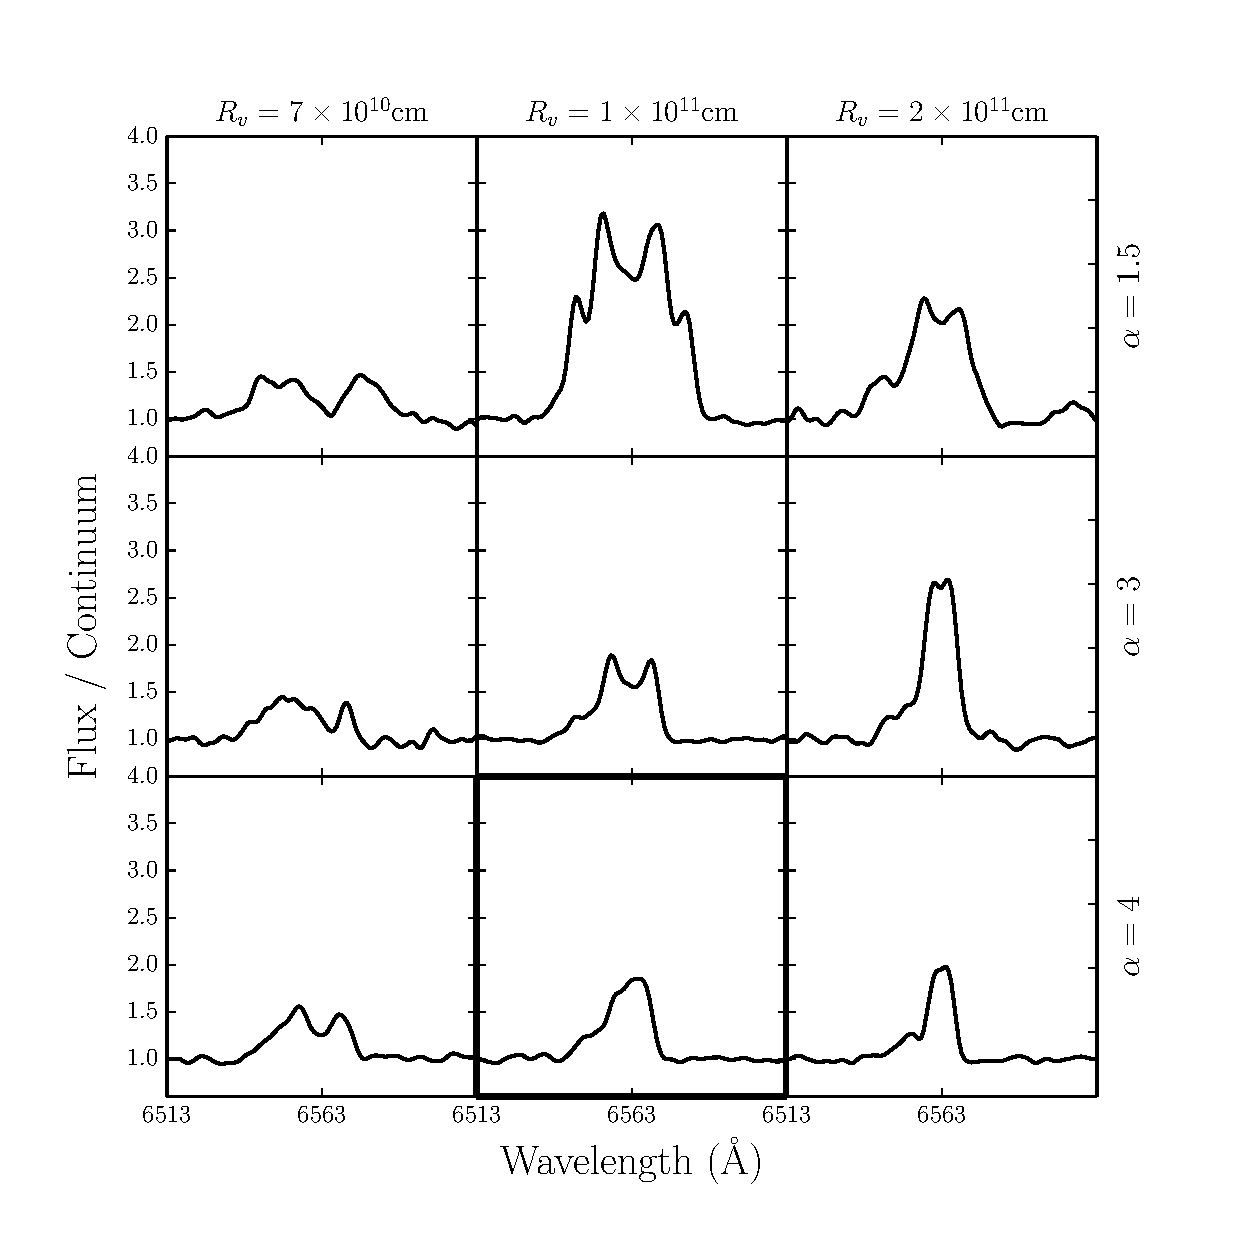
\includegraphics[width=0.5\textwidth]{figures/3by3_grid_alpha.eps}}
\quad
\subfigure{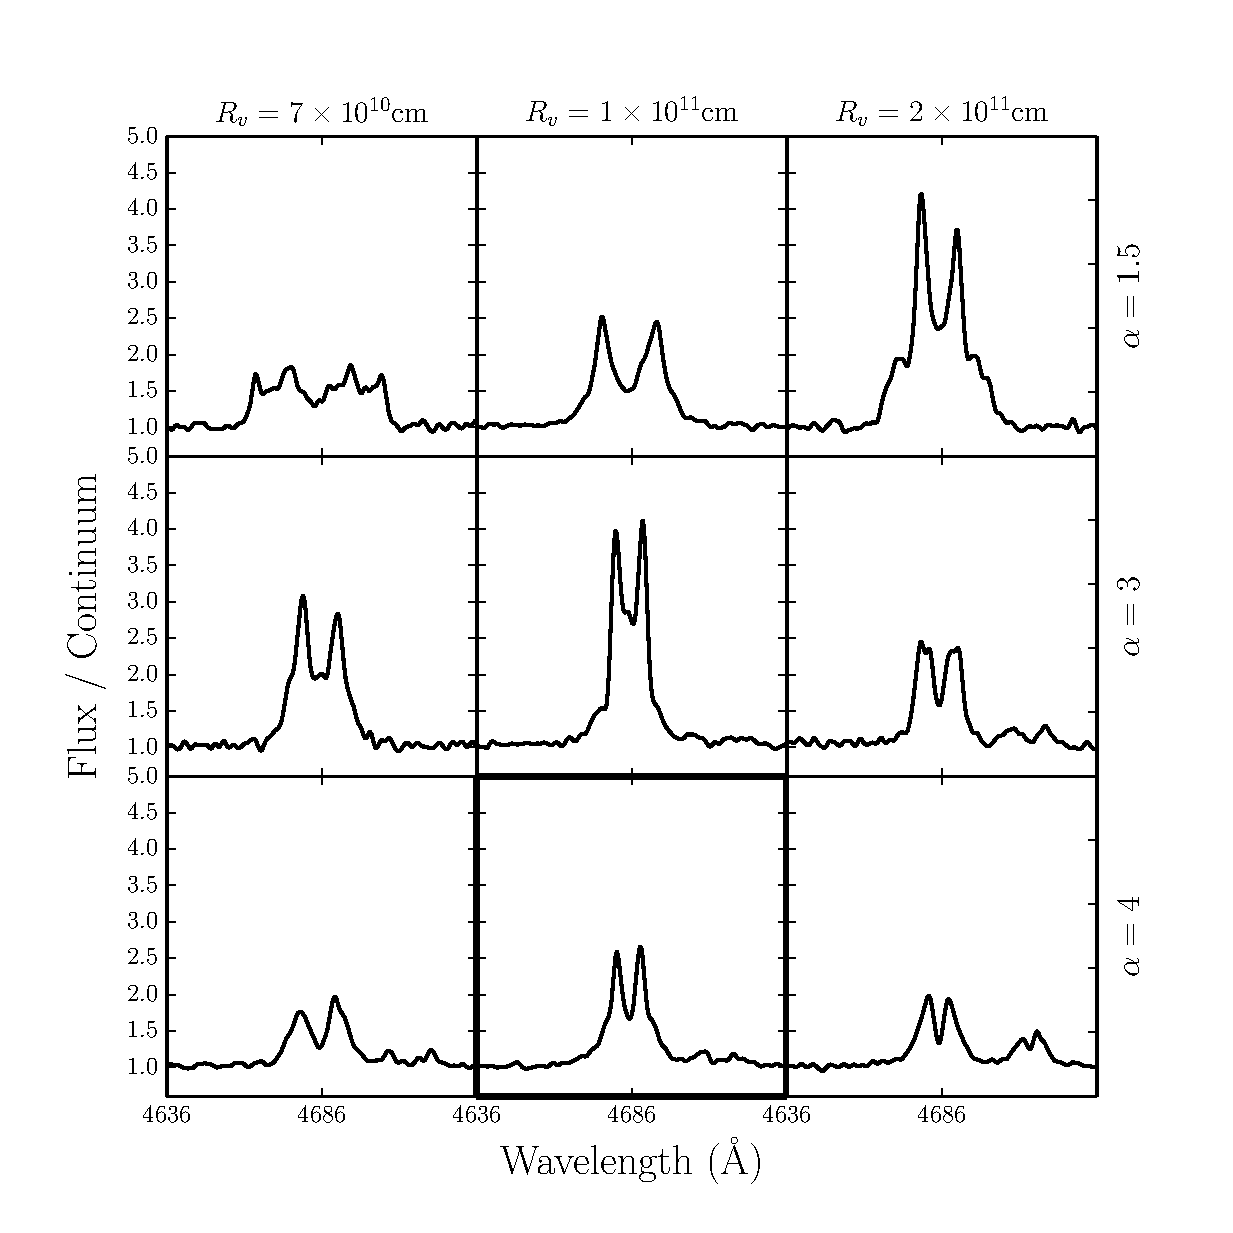
\includegraphics[width=0.5\textwidth]{figures/3by3_grid_4686.eps}}   
}
\caption{
Line profiles plotted in veliocity space 
for \ha\ (left) and \heiiopt\ (right) with varying kinematic 
properties, computed for an inclination of $80^\circ$.
The benchmark model and the improved optical
model described in section 6 are labeled as A and B respectively. 
The $x$-axis limits correspond to the Keplerian velocity at 
$4R_{WD}$, the inner edge of the wind.
The parameter that has been altered from the benchmark model 
is marked in each column and row. Models towards the bottom right
are have more slowly accelerating winds and denser wind bases. 
{\bf JM: Need to discuss the `single-peaked-ness' of line profiles
in our telecon.}
}
\label{halpha}
\end{figure} %fullpage

\begin{figure} %fullpage
\centering
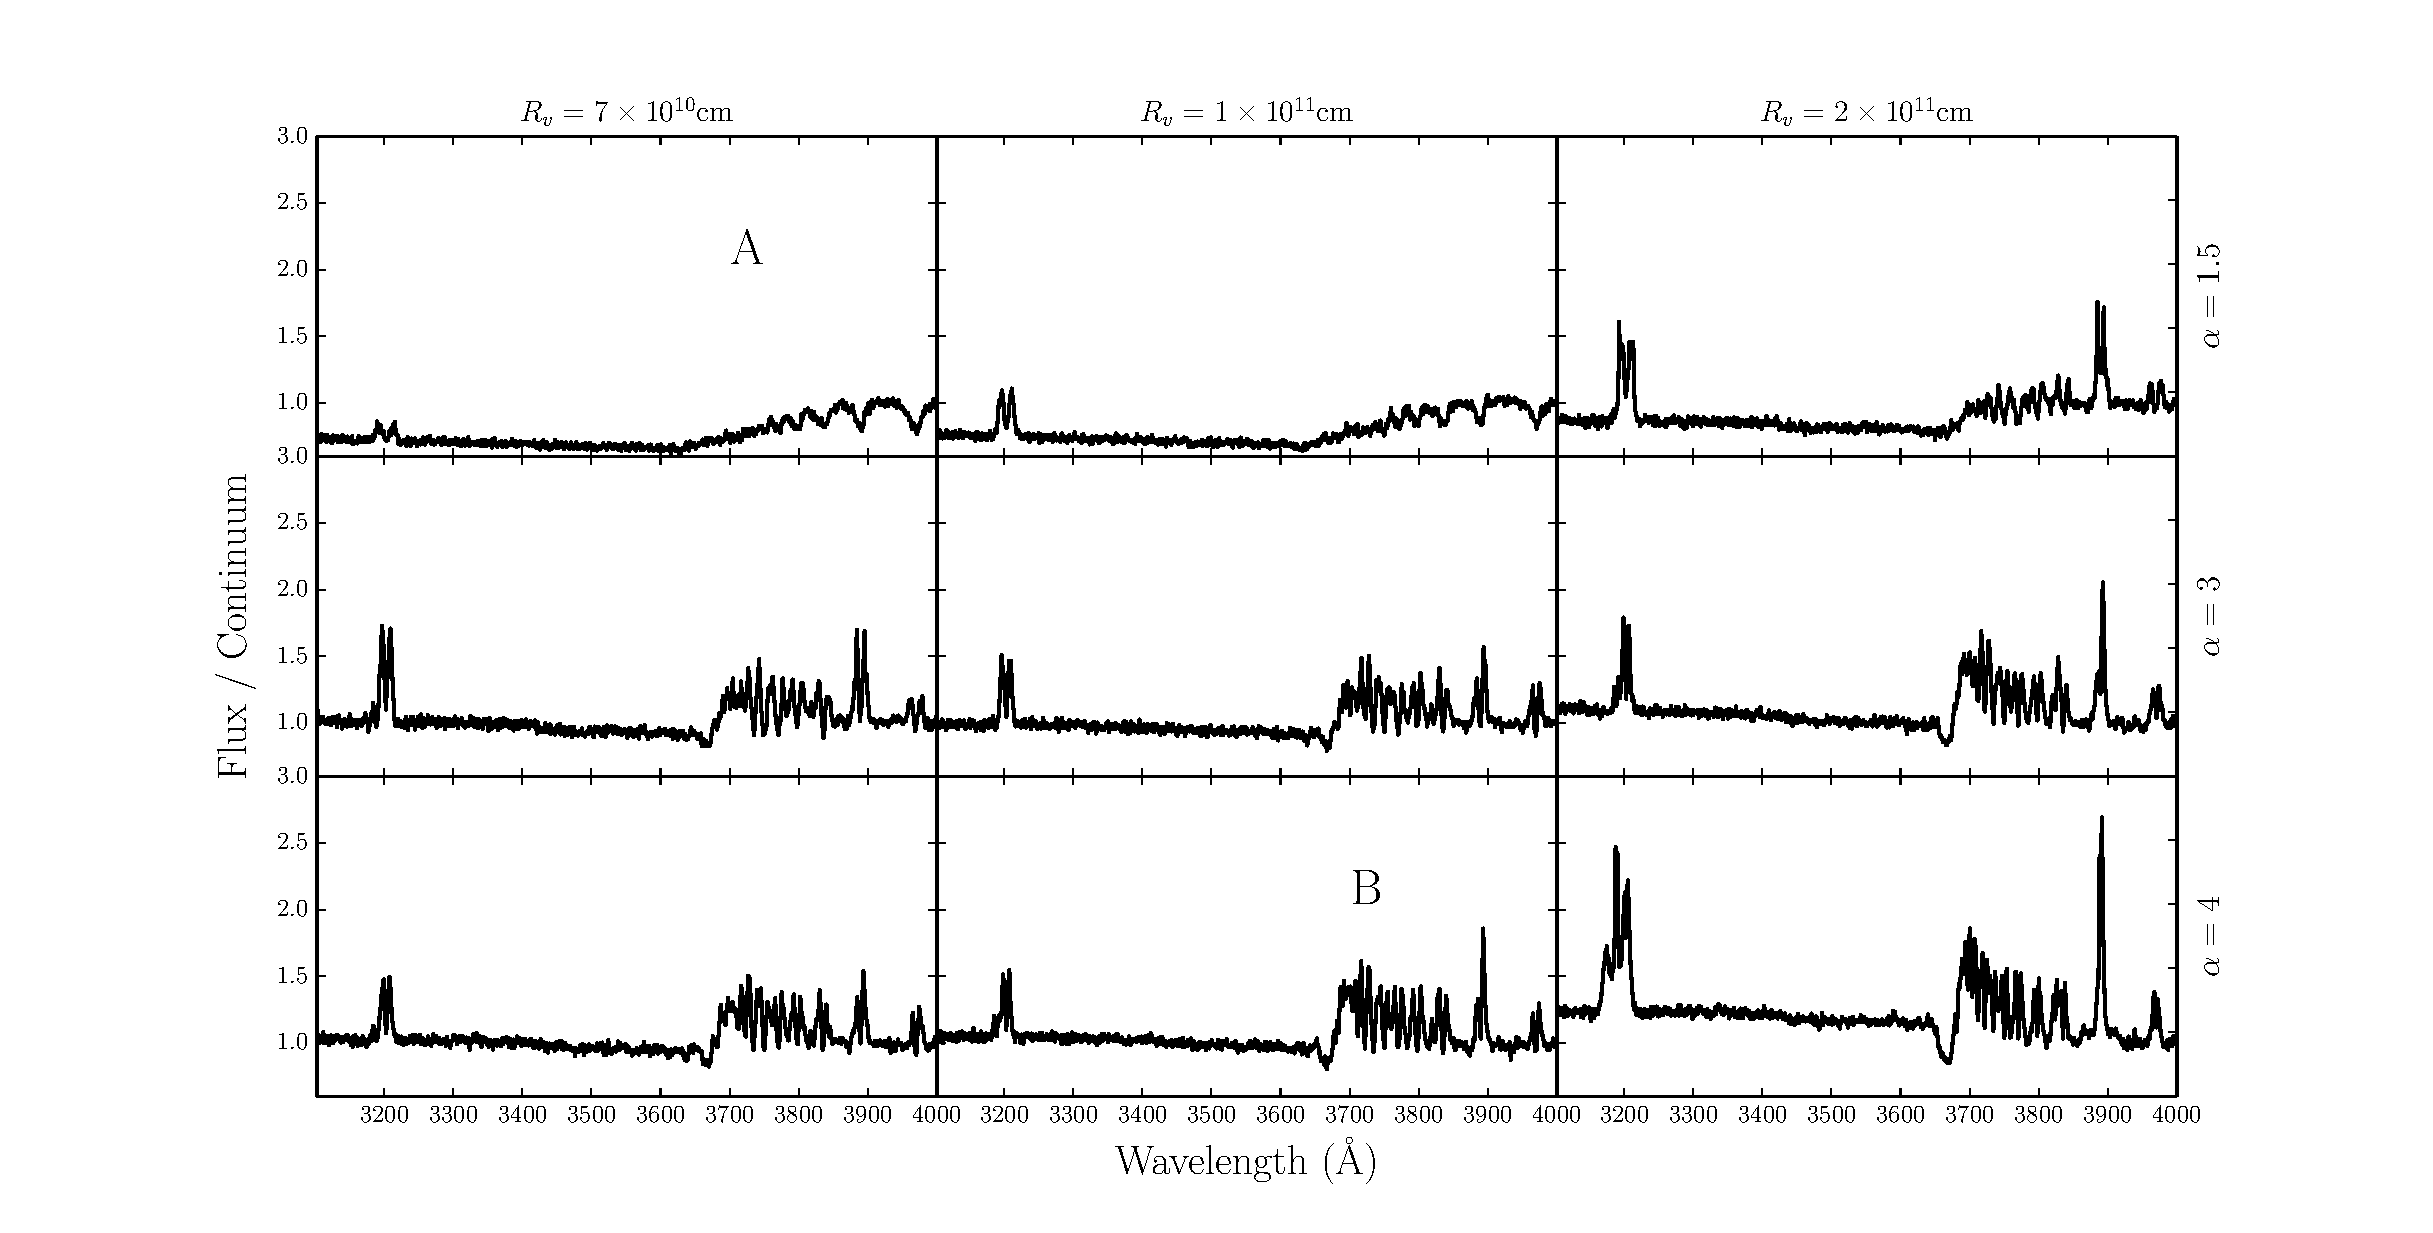
\includegraphics[width=1.0\textwidth]{figures/3by3_grid_balmer.eps}  
%%\includegraphics[width=0.5\textwidth]{figures/test.eps}
\caption{
The evolution of the Balmer jump with varying kinematic 
properties, computed for an inclination of $80^\circ$. 
The panels are organised in the same way as figure~\ref{halpha}.
{\bf JM: Mark lines here?}
% The panels are ordered in the same way as figure~\ref{halpha}. In general, increasing densities
% lead to a Balmer jump in emission, although as in the case of H$\alpha$ there is a transition
% when the wind becomes a neutral absorbing column.
}
\label{jump}
\end{figure} %fullpage

\subsection{Ultraviolet Wind Signatures}
\label{modelb_uv}

The dependence of the ultraviolet C~{\sc iv} and He~{\sc ii} lines on
the same kinematic wind parameters is illustrated in figures~\ref{uvlines}
and~\ref{uvlines}. As before, we focus on the predicted behaviour at $i =
80^\circ$. In our benchmark model, the C~{\sc iv} emission
line seen at high inclinations is almost entirely produced via
resonance scattering. The angle-averaged flux integrated over the
entire line profile - accounting correctly for the blue-shifted
absorption component seen at low inclinations - would be
approximately zero. However, as we increase the density and extent of
the slow-moving part of the outflow near the disk plane, collisionally
excited emission starts to contribute significantly to the C~{\sc iv}
line profiles. This explains the much stronger line-to-continuum
contrast seen in the $\alpha = 1.5$, $R_v = 2\times 10^{11}$~cm model,
for example. For any given inclination, the trend is not necessarily
monotonic, however, because the escape probabilities from the
line-forming region can be highly anisotropic.  
{\bf CK: I *think* this is the basic reason, but (a) can you check
  this, James; (b) is it enough to just point this out?; (c) do we
  understand why CIV is single-peaked but HeII, for example, is double-peaked?
  JM: There are still a few tests I want to do here- we can discuss in the telecon.
  I believe He II v CIV shape is just due to CIV being produced in an extended region,
  and generally scattered, whereas He II is produced close to the disk, and there's probably
  also a line opacity effect.
  I can check this.}

The He~{\sc ii}~1640\AA recombination line is always double-peaked in
our models, although the peak-to-peak separation decreases in the
denser models. For double-peaked lines
formed in rotating media -- in this case, the dense base of the wind
-- the location of the peak(s) is roughly associated with the
projected rotational velocity at the outer edge of the line-forming
region. Thus the trend observed in He~{\sc ii} reflect the radial
expansion of the line-forming region associated with an increase in
the density at the base of the wind. The same trend is actually also
seen in the optical He~{\sc ii}~4686\AA line. The strength of these
features relative to their adjacent continua also track
each other approximately. The reason for the non-monotonic behaviour
in the line strengths as a function of the kinematic wind parameters
is the same as for the C~{\sc iv} line.
{\bf CK: again, can we check this is correct?}

\begin{figure} %fullpage
\mbox{
% \subfigure{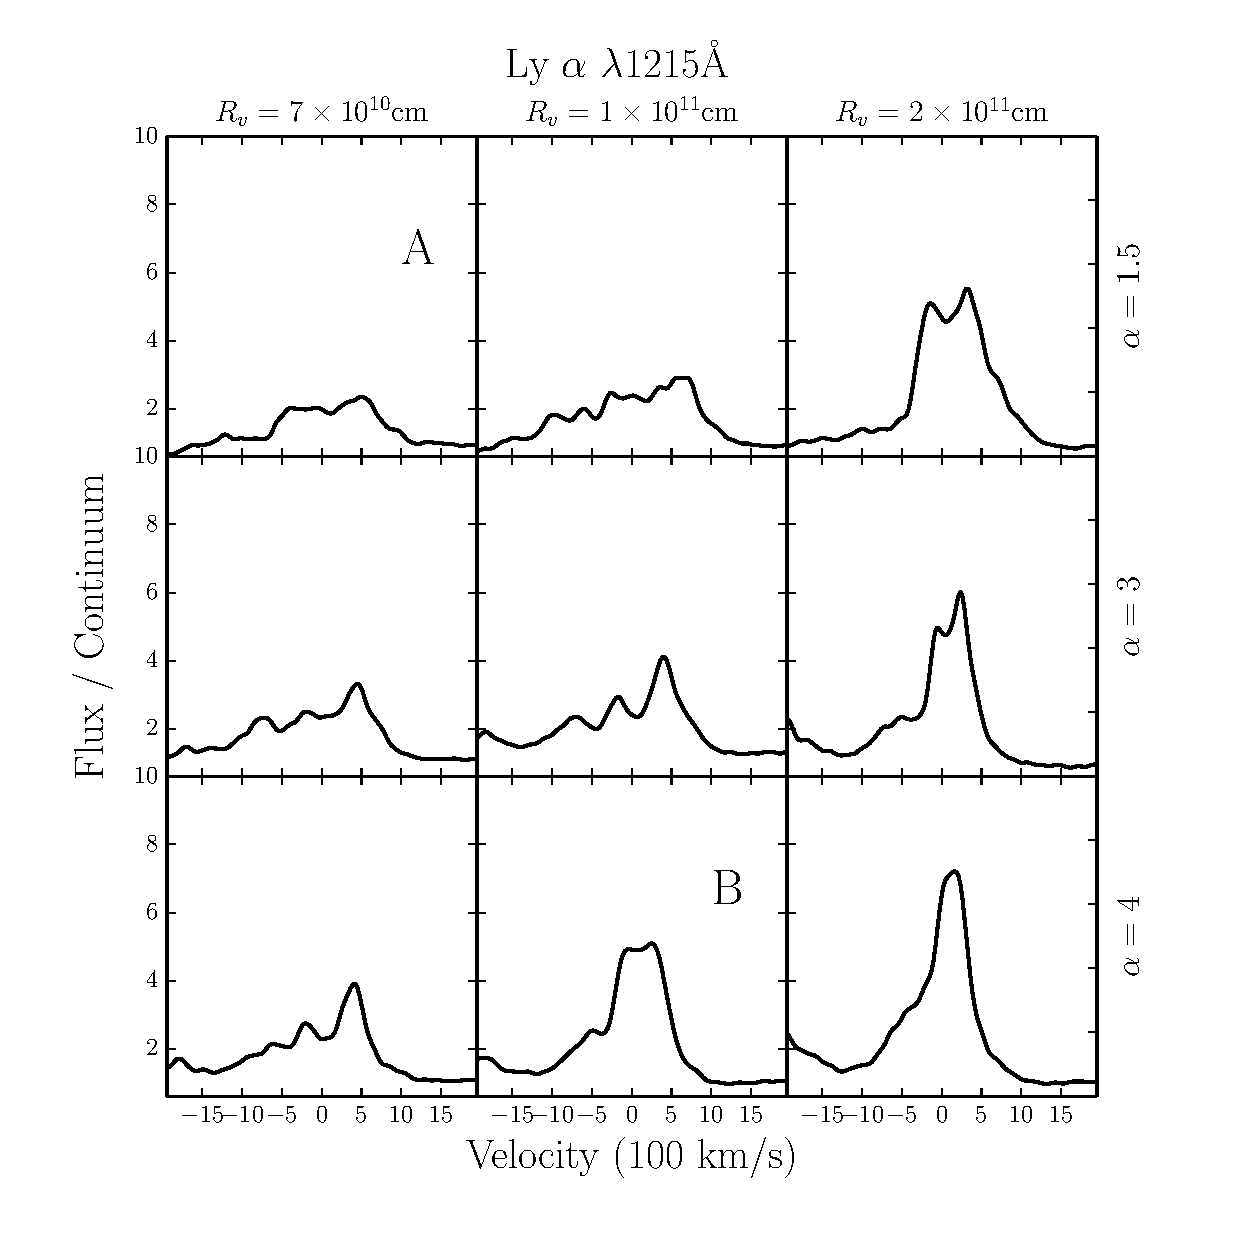
\includegraphics[width=0.33\textwidth]{figures/3by3_grid_lyman.eps}}  
% \quad
\subfigure{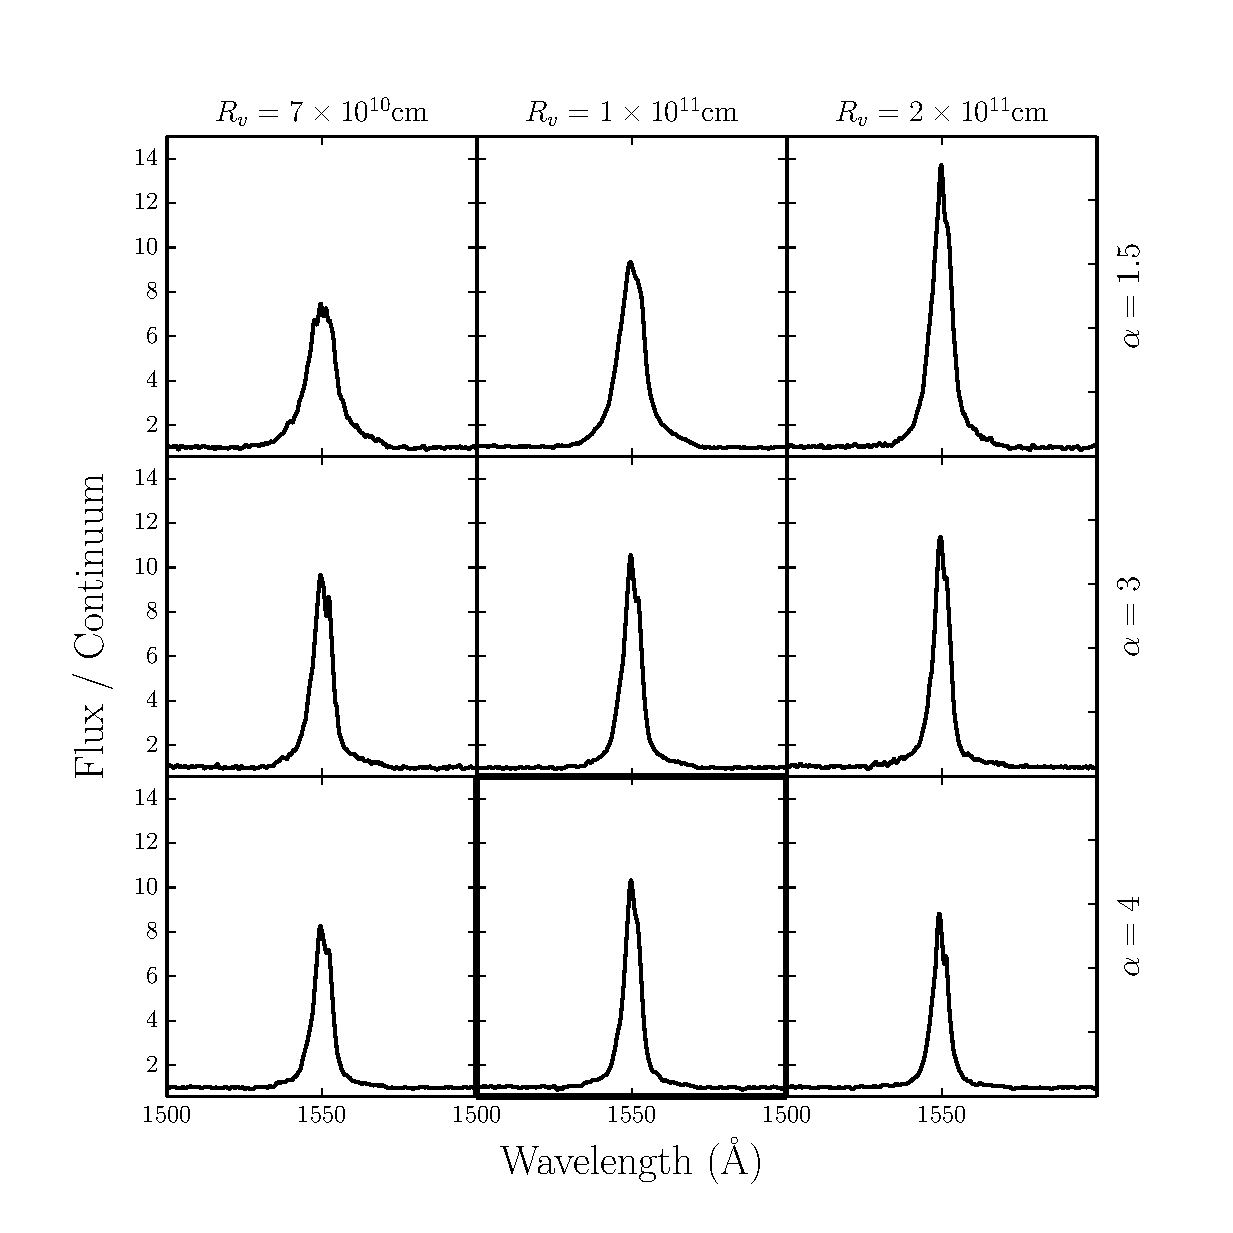
\includegraphics[width=0.5\textwidth]{figures/3by3_grid_uv.eps}}
\quad
\subfigure{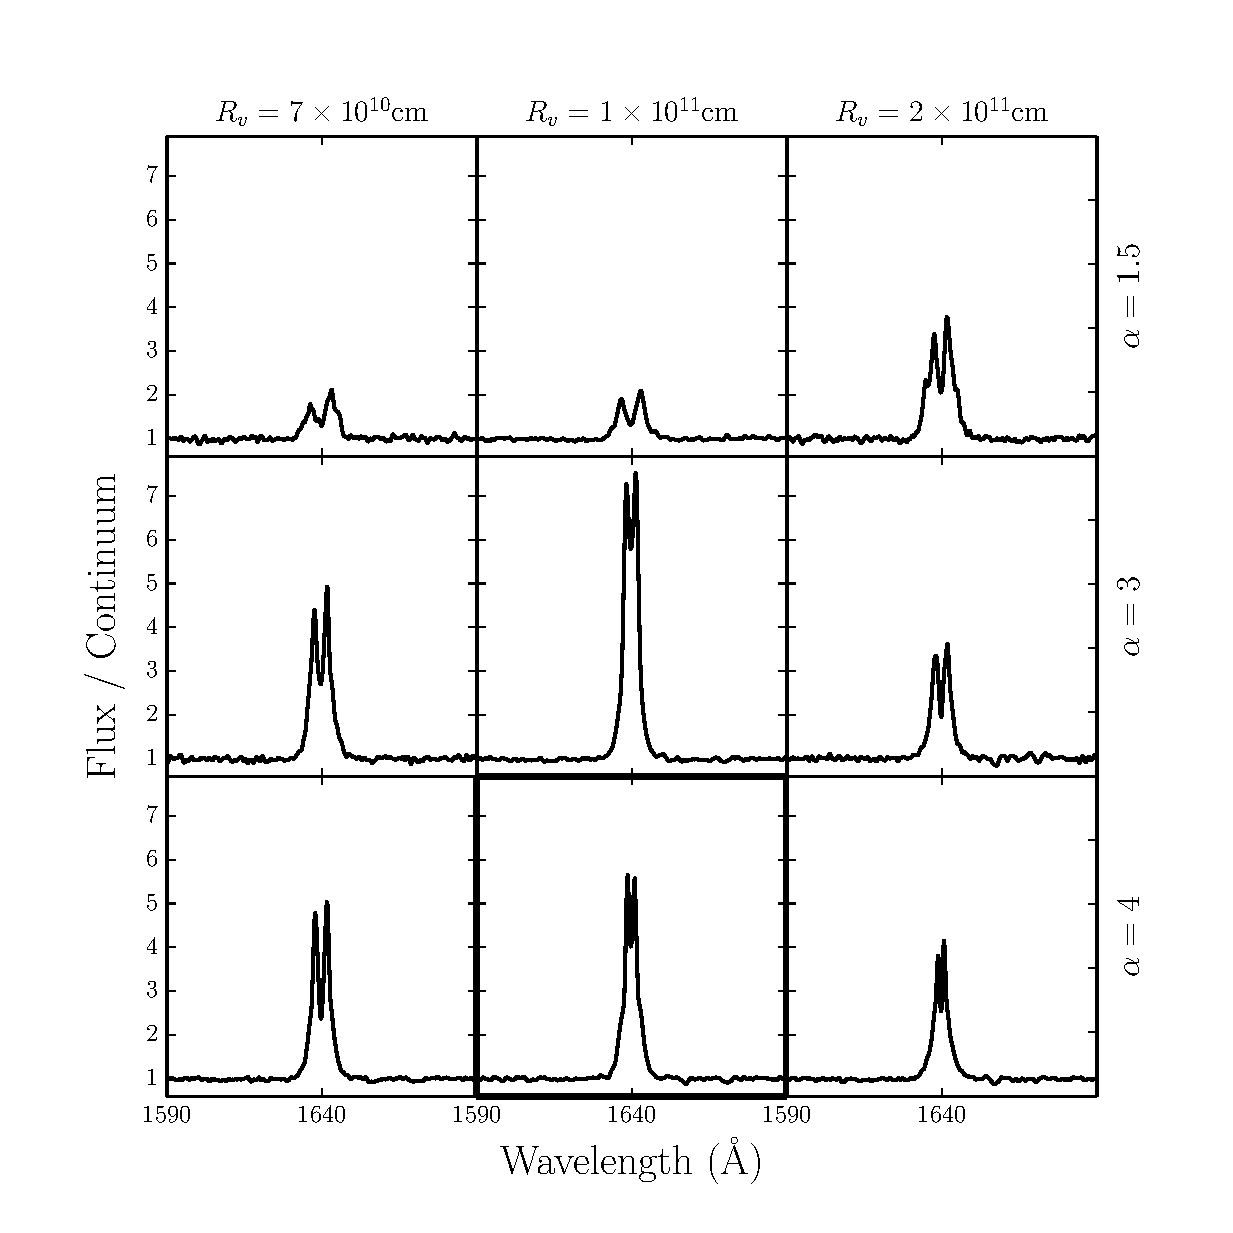
\includegraphics[width=0.5\textwidth]{figures/3by3_grid_1640.eps}}  
}
%%\includegraphics[width=0.5\textwidth]{figures/test.eps}
\caption{
Line profiles for \civ\ (left) and \heiiuv\  (right) with varying kinematic 
properties, computed for an inclination of $80^\circ$. 
The panels are organised in the same way as figure~\ref{halpha}.
{\bf JM: I need to adjust the smoothing here so for all plots I smooth
in terms of Wavelength rather than bins. Linked to single-peaked discussion. 
Note also CK may want a Lyman alpha plot, which I might put here}
% The panels are ordered in the same way as figure~\ref{halpha}. In general, increasing densities
% lead to a Balmer jump in emission, although as in the case of H$\alpha$ there is a transition
% when the wind becomes a neutral absorbing column.
}
\label{uvlines}
\end{figure}


%%%%%%%%%%%%%%%%%%%%%%%%%%%%%%%%%%%%%%
%
%          Comparison with real spectra
%
%%%%%%%%%%%%%%%%%%%%%%%%%%%%%%%%%%%%%%%

\section{A Revised Model Optimized for Optical Wavelengths}

% \begin{table}
% \centering
% \begin{tabular}{p{3cm}p{4cm}}
% Model B\\
% \hline Free Parameters 	&	 Value \\ 
% \hline \hline 
% $M_{WD}$ 	 &	 $0.8 M_{\odot}$ \\ 
% $\dot{M}_{acc}$ 	 &	 $10^{-9}~M_{\odot}yr^{-1}$\\ 
% $\dot{M}_{wind}$  &	$10^{-8}~M_{\odot}yr^{-1}$\\ 
% $r_{min}$ 	&	 $4 R_{WD}$\\ 
% $r_{max}$ 	&	 $12 R_{WD}$ \\ 
% $\theta_{min}$ 	&	 $20.0^{\circ}$ \\ 
% $\theta_{max}$ 	&	 $65.0^{\circ}$ \\ 
% $\gamma$ 	&	 $1$ \\ 
% $v_{\infty}$ 	&	 $3v_{esc}$ \\ 
% $R_v$ 	        &	 $142.9 R_{WD}$ \\ 
% $\alpha$ 	&	 $4$ \\
% \end{tabular}
% \centering
% \caption{Wind geometry parameters used in the revised CV model, Model B,
% which is {\em optimized for the optical band}
% {\bf CK: I actually think we should probably have a single
% table with both sets of model pars}}
% \label{modelb_table}
% \end{table}

The benchmark model discussed in section~\ref{modela} was originally
designed to reproduce the wind-formed lines seen in the UV spectra of
high-state CVs. As we have seen, this model does produce significant
amounts of optical emission. However, with only relatively minor
changes to the kinematics of the benchmark model, it is possible to
construct a model that more closely matches the observed {\em optical}
spectra of CVs (imaginatively dubbed `Model B'). Guided by the results of the previous section, we
adopt the parameters listed in table~\ref{modelb_table} for this purpose.

Figure~\ref{uvoptb} shows the predicted UV and optical spectra for this
optically optimized model for the full range of inclinations, and
Figure~\ref{rwtricomp} shows a qualitative comparison of the predicted
out-of-eclipse and mid-eclipse spectra against observations of the
high-inclination nova-like RW~Tri. The inclination of RW Tri is
somewhat uncertain, with estimates including $70.5^\circ$
\citep{smak1995}, $75^\circ$ \citep{groot2004}, $80^\circ$
\citep{longmore1981} and $82^\circ$\citep{frankking1981}. Here, we
adopt $i = 80^\circ$, but our qualitative conclusions are not
particular sensitive to this particular value. We emphasize that this
model is in no sense a fit to this -- or any other -- data set.
{\bf CK: strictly speaking, we should be talking about q=M2/M1 and disk
  radius here as well I think, since those parameters affect the
  amount and nature of any uneclipsed light just as much (sort of) as
  the inclination. We should probably quote M2, q and R2/a in the
  table, and we may want to say that we've adopted a q that is in line
  with the observed eclipse width of RW Tri. (In Roche geometry,the
  eclipse width -- the half-width at half out-of-eclipse intensity,
  say -- depends solely on q and i). See e.g. Horne's paper or various
  Dhillon et al. papers.}

The similarity between the synthetic and observed spectra is
striking. In particular, the revised model produces strong emission in
all the Balmer lines, with line-to-continuum ratios comparable to
those seen in RW Tri. Moreover, the line-to-continuum contrast
increases during eclipse, as expected for emission produced in a disk
wind. This trend is in line with the observations of RW~Tri, and it
has also been seen in other NLs, including members of the SW~Sex class
(REF) {\bf CK: I'm pretty sure that we know this about UX Uma, e.g. from
  eclipse mapping studies, and there ought to be mid-eclipse spectra
  of some additional system}
The revised model also produes a single-peaked \ha\ line, in line with
the observational data.

However, there are also interesting differences between the revised
model and the RW Tri data set. For example, H$\alpha$ is the only line
that is single-peaked in the model, in contrast to what is seen in the
observations. (However, the relatively low resolution of the RW Tri
spectra makes this comparison difficult.) Moreover, the model exhibits
considerably stronger He~{\sc ii} features than the observations,
which suggests that the overall ionization state of the model is
somewhat too high. 

However, perhaps the most serious problem for this optically optimized
model is associated with its predicted UV spectra. In order to
generate strong optical wind signatures, we have adopted wind
parameters that lead to very high densities at the base of the wind
($n_e\sim10^{13}-10^{14}$ in the main emission region). This produces
the desired optical recombination emission, but also increases the
role of collisional excitation in the formation of the UV resonance
lines. This explains the pronounced increase in the emission component 
of the C\textsc{iv} 1550\AA resonance line, for example, relative to
what was seen in the benchmark model (compare figures~\ref{spec} and
\ref{uvoptb}). The strength of this component in the revised model --
especially at low and intermediate inclinations -- is probably
somewhat too high to be consistent with UV observations of high-state
CVs (REF).

\begin{figure} %fullpage
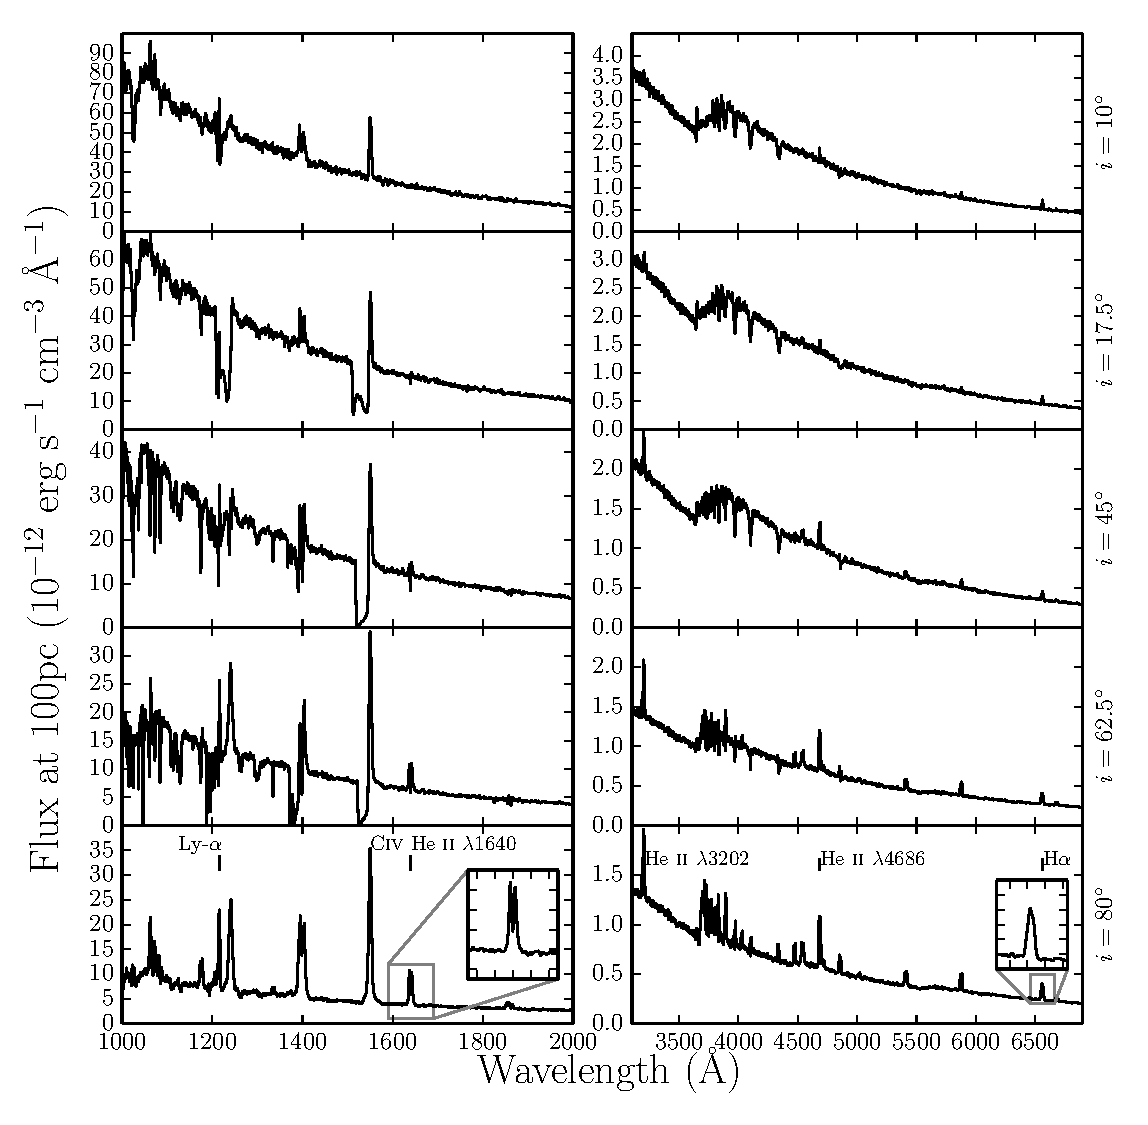
\includegraphics[width=\textwidth]{figures/fig14_uv_opt.eps}
\caption{
UV (left) and Optical synthetic spectra for model B computed at
sightlines of 10, 27.5, 45, 62.5 and 80 degrees.	
The inset plots show zoomed-in line profiles for 
\heiiuv\ and \ha. The \ha line 
is single peaked, but higher order lines in the Balmer series
are double-peaked, albeit with narrower profiles.
Strong \heiiopt\ emission can be seen, as well a trend
of a deeper Balmer jump with decreasing inclination.
}
\label{uvoptb}
\end{figure} %fullpage


\begin{figure} %fullpage
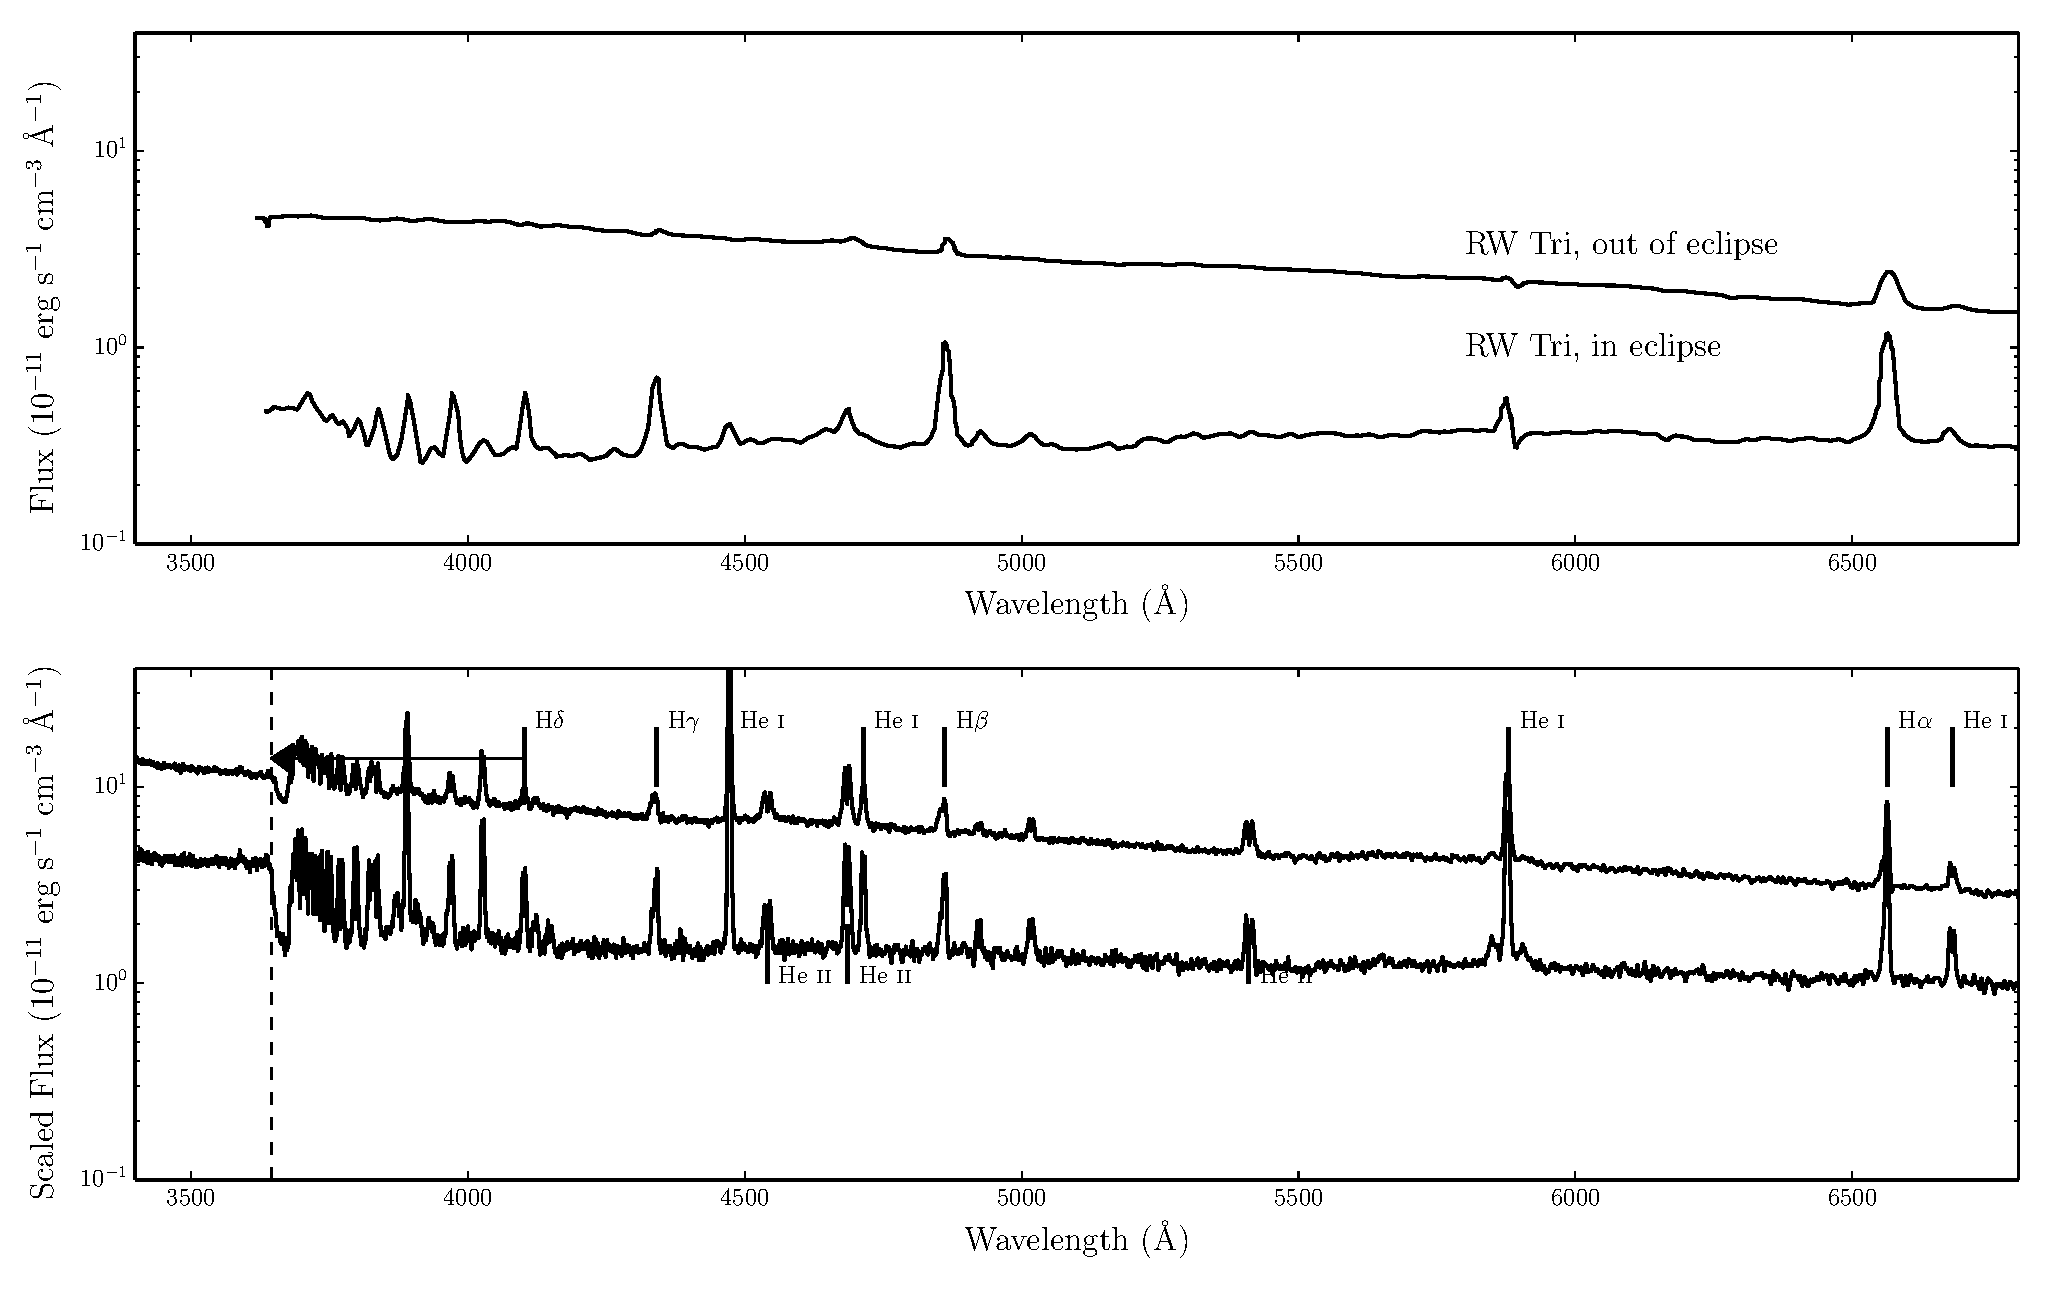
\includegraphics[width=0.8\textwidth]{figures/fig13_eclipse.eps}
\caption{{\sl Top Panel:} In and out of eclipse spectra of the high
inclination NL RW Tri. {\sl Bottom Panel:} In and out of eclipse synthetic
spectra from Model B.
The artificial `absorption' feature just redward of the Balmer jump
is caused for the reasons described in section 5.2.}
\label{rwtricomp}
\end{figure} %fullpage


% \noindent\rule{16cm}{0.4pt}

% {\bf
% \noindent Notes on Section 6:

% \begin{itemize}
% 	\item 

% \noindent Potential Additional Figures:

% \begin{itemize}
% 	\item 	
% }

% \noindent\rule{16cm}{0.4pt}

%%%%%%%%%%%%%%%%%%%%%%%%%%%%%%%%%%%%%%
%
%          Conclusions and Future Work
%
%%%%%%%%%%%%%%%%%%%%%%%%%%%%%%%%%%%%%%%


\section{Conclusions}

We have investigated whether a disk wind model designed to reproduce
the UV spectra of high-state CVs would also have a significant effect
on the optical spectra of these systems. We find that this is indeed
the case. In particular, the model wind produces H and He
recombination lines, as well as a recombination continuum blueward of
the Balmer edge. 

We have also explored the dependence of the optical (and UV) wind
signatures on some key kinematic wind parameters. Based on this, we
show that recombination emission from outflows with sufficiently high
densities and/or optical depths might 
\renewcommand{\labelitemi}{$\bullet$}
\begin{itemize}
	\item fill in the Balmer absorption edge in the spectrum of
          the accretion, thus accounting for absence of this edge in
          observed CV spectra\citep{KLWB98};
	\item produce the commonly observed single-peaked optical line
          profiles \citep{MC96}
\end{itemize}
\smallskip

{\bf JM: I originally also had a note about the flat Balmer decrement here.
it's potentially interesting and could be included, but would need a discussion
earlier in the text.}


\noindent Based on our modelling, we can also make a number of basic,
testable predictions for wind-formed signatures:
\begin{itemize}
	\item we expect the depth of the Balmer absorption edge in CV
          spectra to decrease with increasing inclination (with the
          Balmer jump possibly switching to emission at the highest
          inclinations, if the flux in the wind-formed recombination
          continuum exceeds that of the foreshortened disk spectrum);
	\item we predict that a strong He~\textsc{ii}~$\lambda3202{\rm
          \AA}$ line should be prominent in all cases where
          He~\textsc{ii}~$\lambda1640{\rm \AA}$ \& \heiiopt\ are seen
          (but note that this prediction is not restricted to lines
          formed in disk winds);
	\item we predict that the Balmer jump should be in emission
          during mid-eclipse in high inclination systems.
\end{itemize}

\smallskip
We have also constructed a revised benchmark model which is designed
to more closely match the optical spectra of high-state CVs. This
optically optimized model produces all the prominent optical lines in
and out of eclipse, and achieves reasonable verisimilitude with the
observed optical spectra of RW Tri. However, this model also has
significant shortcomings. In particular, it predicts
stronger-than-observed He~{\sc ii} lines in the optical region and too
much of a collisionally excited contribution to the UV resonance lines
that  

Overall, our work demonstrates that {\sl disk winds matter}. They are
not just responsible for creating the blue-shifted absorption and
P-Cygni profiles seen in the UV resonance lines of high-state CVs, but
can also have a strong effect on the optical appearance of these
systems. In fact, most of the optical features characteristic of CVs
are likely to be affected -- and possibly even dominated -- by their disk
winds. Given that optical spectroscopy plays the central role in
observational studies of CVs, it is clearly critical to know 
where and how these spectra are actually formed. We believe it is high
time for a renewed effort to understand the formation of spectra in
accretion disks and associated outflows. 

{\bf CK: I just realized that -- apart from the intro -- we never
actually discuss the issue of P Cyg profiles in the optical
lines. These have been observed -- e.g. in Halpha -- but I guess we
never produce these? Do we know why? We probably should at least
comment on this at some point in the text, and possibly even briefly
in the conclusions.}

%% Balmer jump

% {\bf
% \noindent Notes on Section 7:

% \begin{itemize}
% 	\item 

% \noindent Potential Additional Figures:

% \begin{itemize}
% 	\item 	
% }


% \subsection{Future Work}

% To further investigate the true effect of the wind
% we hope that high quality, broadband spectra of 
% Nova-like variables at a range of inclinations 
% will be taken to examine 

% In addition to this project, we have started to apply the macro atom scheme to QSOs in order to build on the work of Higginbottom et al. (2013). In particular, we hope that the macro-atom scheme will enable the
% model to produce significant Lyman-$\alpha$ emission, as is observed in QSOs.


\subsection*{Acknowledgements}
The work of JHM, NH and CK is supported by the Science and Technology Facilities Council (STFC), 
via studentships and a consolidated grant, respectively. We would like to thank Juan Hernandez Santisteban and Ivan Hubeny 
for useful discussions. We acknowledge the use of the IRIDIS High Performance Computing Facility, 
and associated support services at the University of Southampton, in the completion of this work.


\newpage
\newpage
\bibliography{mybib.bib}

\end{document}
